\chapter{Results and Discussion} \label{chap:3}

    \section{Rating of clustering quality}
    
    \subsection{Detailed vectorization}
    
    Execution of the \textit{rating.sh} script was performed on the files generated in the used pipeline (\autoref{chap:2}), containing the clustering tools and their related clusters, as well as the representatives of the clusters and the sequences in the clusters. In \textit{rating.sh}, the sequences related to the cluster were extracted from a \gls{msa} and converted to a frameshift-, gap, and \gls{ORF}-aware sequence difference vector, by a python script named \textit{vectorize.py} (\autoref{fig:3.2}). 
    
    To calculate these vectors, the following procedure was performed once for every sequence in the cluster, as well as once for the clusters representative. First the gaps were removed from the strand, resulting in the original sequence before the alignment. Following the removal, the \gls{ORF} of the sequence was extracted by starting from the first nucleotide and proceeding in triplets, until a start codon was found. The nucleotides following the start codon were saved while counting the length of the \gls{ORF}. When a stop codon was found, the sequence from start to stop was saved in a second variable and the first one was emptied. Read-in of the triplets proceeded until a new start codon was found, from which on the sequence was saved again in the emptied first variable, while the length was counted again. Only if the second sequence from start codon to stop codon was longer than the first one, the second variable was emptied and filled by the second found sequence. The same procedure was repeated until the whole strand was searched for every possible \gls{ORF}. The longest \gls{ORF} and its related candidate nucleotide sequence was then saved in a third variable. Furthermore, a second and third candidate sequence was searched by shifting the triplets by one and two and repeat the process again. Finally the longest candidate was accepted as the most likely \gls{ORF} related to this sequence in the cluster and finally saved.
    
    With the found \gls{ORF} sequence in mind, the length of the 5'-\gls{UTR} and 3'-\gls{UTR} were calculated. The saved \gls{ORF} sequence was converted to a list of single nucleotides. Every nucleotide from the list was then replaced by its related \gls{AA}, e.g., the nucleotides \textit{A}, \textit{U}, \textit{G} were replaced by methionine. Single gaps were afterwards added to the start of the list, their number according to the length of the 5'-\gls{UTR} nucleotides and likewise added to the end of the list matching the 3'-\gls{UTR} length. The previous removed gaps were also included at their exact removed positions. In conclusion, the procedure created a list reflecting a related \gls{AA} to every nucleotide of the strand if the nucleotide was in the \gls{ORF} or otherwise a gap (\autoref{fig:3.2} bottom left). This more complex approach served the conservation of related \glspl{AA} to the single nucleotides in case of frameshifts, gaps in the triplets, and longer or shorter \glspl{UTR}.
    
    \begin{figure}[!htb]
        \centering
        \fbox{\includegraphics[width=\dimexpr\textwidth-2\fboxsep-2\fboxrule, page=3]{Figures/Projektarbeit_Tikz.pdf}}
        \caption[Detailed procedure of \textit{vectorize.py}]{\textbf{Detailed procedure of \textit{vectorize.py}.} For the rating of clustering quality %\
        %DD{Hier sollte etwas mehr Figure Text sein. Am bessten alles auf dem Bild kurz beschreiben, also die einzelnen Steps.}
        the representative of the cluster, as well as the sequence $n$ was extracted from the previous generated \gls{msa}. Gaps in both sequences were removed and the \glspl{AA} in the {ORF} annotated to the related nucleotides. With information of the \glspl{AA} in mind, both sequences from the \gls{msa} were compared nucleotide-wise for no change, transition, insertion, deletion, transversion or silent mutation and rated accordingly in the sequence difference vector. This process was repeated for every sequence $n$ of the cluster.}
        \label{fig:3.2}
    \end{figure}
    
    The procedure was first performed on the representative and then iteratively for every sequence in the cluster. After the procedure was finished for the first sequence of the cluster, there were two sequences from the \gls{msa}, one for the representative and one for the first cluster sequence, as well as two lists representing their \glspl{AA} constellation. The first vector of sequence difference was then calculated by simultaneously iterating the two \gls{msa} sequences. If the nucleotides matched, the value zero was saved in the vector at the same position as the nucleotide. If the nucleotides did not match, the related positions in the two lists were compared for the same \gls{AA} and by success rated with the value one. If there was still no match, the two \gls{msa} sequences were compared for transition at the position (A $\leftrightarrow$ G or U $\leftrightarrow$ C) and rated with the value two. Insertion, deletion, or all other types of \glspl{SNP} were rated by the value three (the highest penalty). After the first vector was finished, only the \gls{msa} sequence and list for the first cluster sequence were deleted and the process started again, for the next cluster sequence. \Gls{msa} sequence and list for the representative were kept for the next comparison. 
    
    The substitution matrix used in the process was build by considering evolutionary aspects (insertion, deletion, transversion, transition, silent mutations), to assign nucleotide differences with specific scores, for a reasonable estimation of the clustering quality \autocite{matrix}. Despite that, the rating process was build for easy customization in mind. The components were build to allow a way more complex transition table instead, by only changing some lines in the script pipeline. While calculation of the penalty, the nucleotide of the representative and sequence as well as the related triplet of the representative and sequence are available and considered. By changing the penalty calculation from the simple progressive if checkback to a lookup of the four components in a more specific transition table, a more accurate rating can be accomplished and the pipeline can be modified for specific questions. 
    
    \subsection{Run time estimation of the rating process}
    
    Under the assumption that the used \gls{msa} of the genomes from segment $X$ contains $m$ sequences of length $o$ and the cluster to be rated contained $n$ of these sequences, the duration was calculated as follows:

    \[ m \cdot (n + 1) + 6 \cdot o \cdot ( n + 1 ) + 2 \cdot o \cdot n + n^2 = O(n(m+n+o))\]
    
    Every sequence in the cluster was extracted from the \gls{msa} once. The clusters representative instead twice, as a normal sequence in the cluster and as the clusters representative to compare the other sequences with. This resulted in
    
    \[ m \cdot (n + 1) = O(m\cdot n) \]
    
    operations. 
    
    All extracted sequences an the representative ($n+1$) were lapsed six times to remove the gaps, search for the \gls{ORF} three times (to search in every shifting possibility), annotate the \glspl{AA} and restore the gaps:
    
    \[ 6 \cdot o \cdot (n + 1) = O(o\cdot n) \]
    
    For the calculation of the sequence to the representative difference vector, every sequence was lapsed once together with the representative, so
    
    \[ 2\cdot o \cdot n = O(o\cdot n) \]
    
    operations were needed.
    
    Finally, the distance between every vector to every other vector was calculated:
    
    \[ n^2 = O(n^2) \]
    
    The segment wise rating of the clustering quality of three tools for eight segments from \gls{IBV} with 500 sequences took less than five minutes.
    
    \subsection{Implementation of step and window size}

    Investigation of the possibility to use window and step sizes to reduce calculation time in the distance calculation was carried out by rating the same cluster from CD-HIT, usearch and VeGETA repeatedly with different sizes. In detail, the penalty of the nucleotides in the window was summed up to reduce the vector size and then iteratively shifted by the step size. The distance function in the R script calculated the distance between every vector in the cluster to each other, therefore, a reduction of the calculation time by shrinking the vector size was expected. By coloring of the resulting \glspl{MED} based on the used step and window sizes, the clustering quality of the tools with different settings could be observed (\autoref{fig:3.1}). Changing the step and window sizes for calculation on the same cluster resulted only in a change of the resulting \gls{MED} magnitude, but did not change the quality the slightest, since the quality difference from tool to tool was preserved. While this result reflected the expected robustness of the rating script, the change in window and step size unexpectedly did not reduce the duration of the calculation. Instead, the calculation time was increased slightly due to the double calculation of penalties in the overlapping area of window and step size, since every window was calculated one by one. In conclusion, the vector calculation step was the run time determining one, instead of the vector distance calculation. By keeping this in mind, the implementation for step and window size was declared obsolete and removed.

    \begin{figure}[!htb]
        \centering
        \fbox{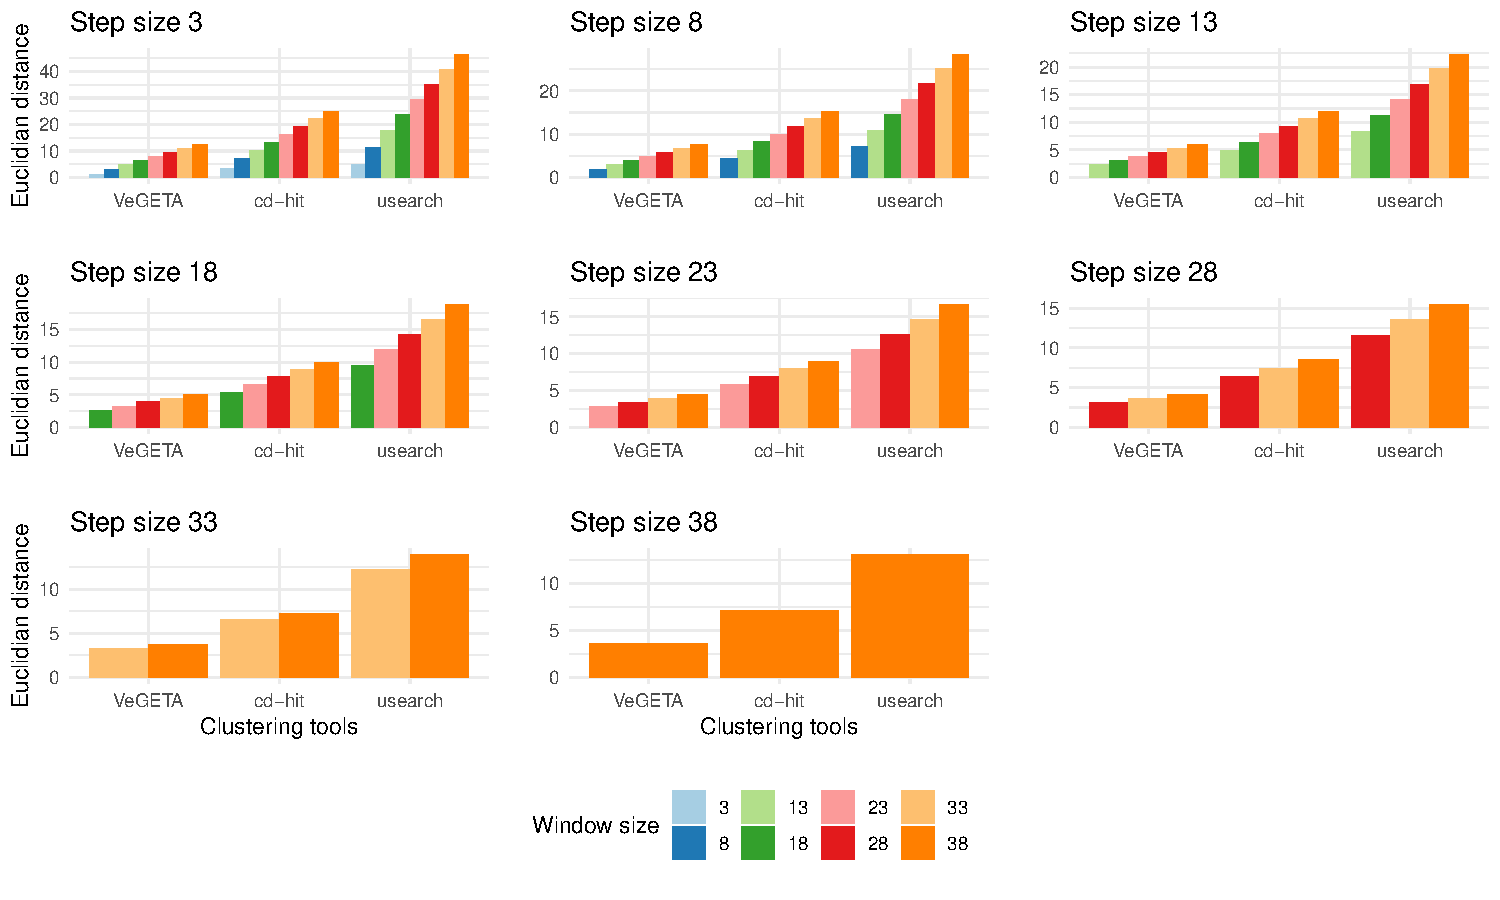
\includegraphics[width=\dimexpr\textwidth-2\fboxsep-2\fboxrule]{Figures/Step.pdf}}
        \caption[Window and step size]{\textbf{Window and step size.} Comparison of different used step and window sizes in combination with the rating pipeline. Euclidean distance was used for the vector comparison only. Step size can only be less equal to the window size to prevent skipping nucleotides in the rating process. Clustering quality of the used tools can be compared in the same window and step sizes.}
        \label{fig:3.1}
    \end{figure}
    
    \subsection{Comparison of distance functions}
    
    For the best possible cluster rating, the results of the \textit{rating.sh} were calculated with euclidean and with manhattan distance function. The best clustering tool was chosen by having the least distance (\gls{MED} with euclidean function and \gls{MMD} with manhattan function). While the comparison of the used functions in the results of the rating for all the segments of \gls{IBV} (\autoref{fig:3.7} and \autoref{fig:3.8}) showed mostly similar behavior, with a change in magnitude, the results for segment three and four differed (exact distance values in \autoref{tab:A.1}). This was explained by the calculation of the distance function and the resulting stronger impact of the higher distance of single sequence clusters in the \gls{MMD}. While single sequence clusters should increase the overall distance to impair the tool in the ranking, the increasing of \gls{MMD} by single sequence clusters was disproportionate. For the use of \gls{MMD} as distance, the weighting of single sequence clusters should be reconsidered. While the using of \gls{MMD} may overestimate the penalty of single sequence clusters, VeGETA still seemed to have the overall lowest distance in both methods, with exception of segment three and four with with the \gls{MMD}. 
    
    \begin{figure}[!htb]
        \centering
        \fbox{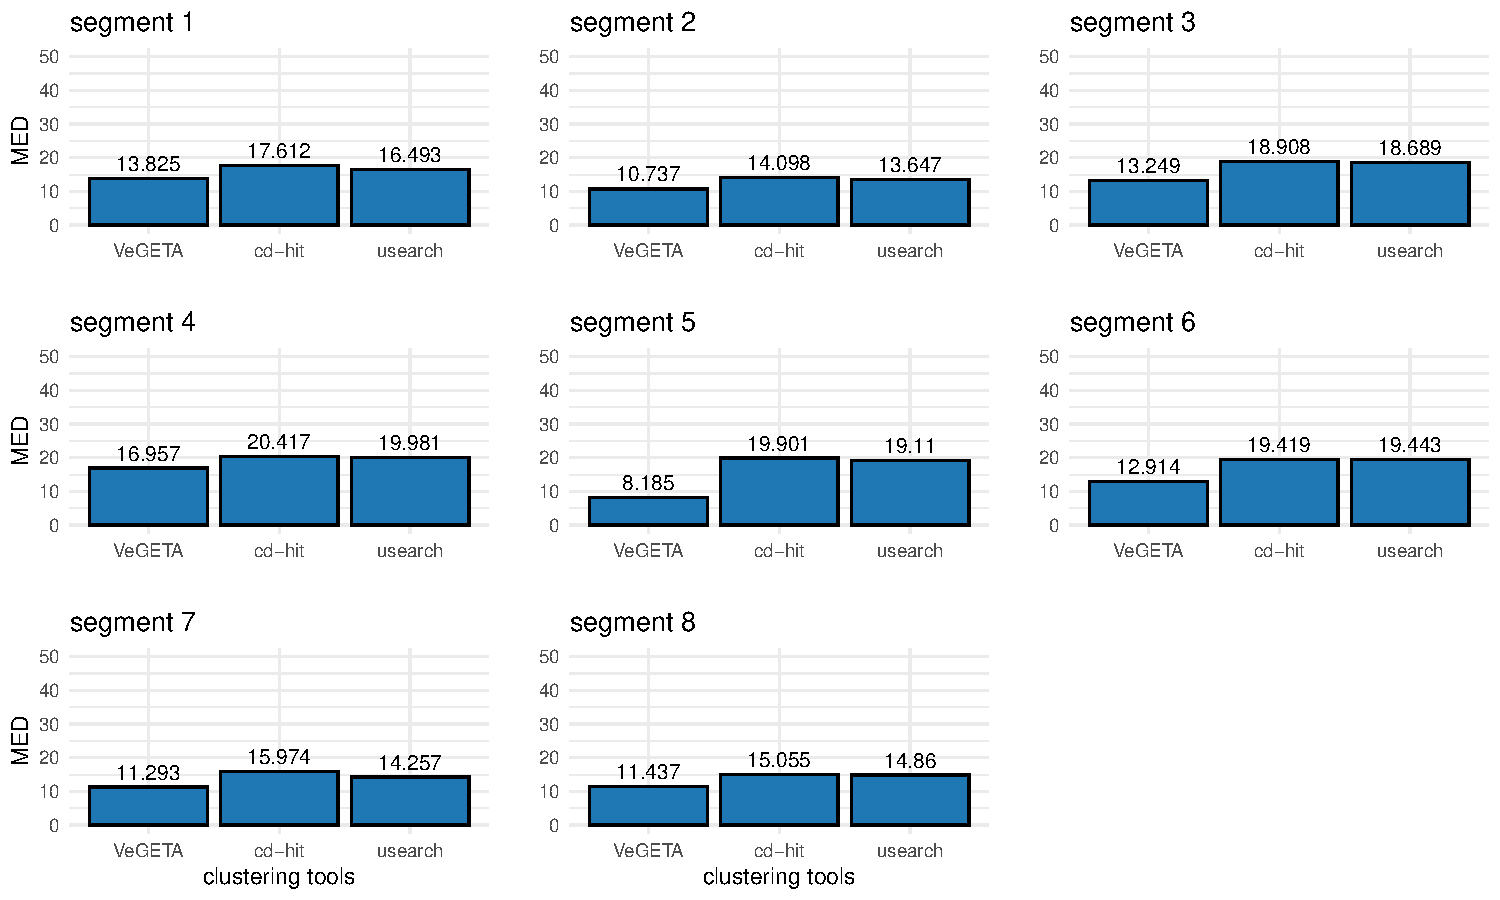
\includegraphics[width=\dimexpr\textwidth-2\fboxsep-2\fboxrule]{Figures/Seg_MED.pdf}}
        \caption[Clustering quality of all segments measured with \gls{MED}]{\textbf{Clustering quality of all segments measured with \gls{MED}.} For all segments of \gls{IBV} the rating pipeline with \gls{MED} as measurement was used to rate the quality of the clusters generated by CD-HIT, usearch and VeGETA. The distances are weighted by the cluster sizes generated by the tools.}
        \label{fig:3.7}
    \end{figure}
    
    \begin{figure}[!htb]
        \centering
        \fbox{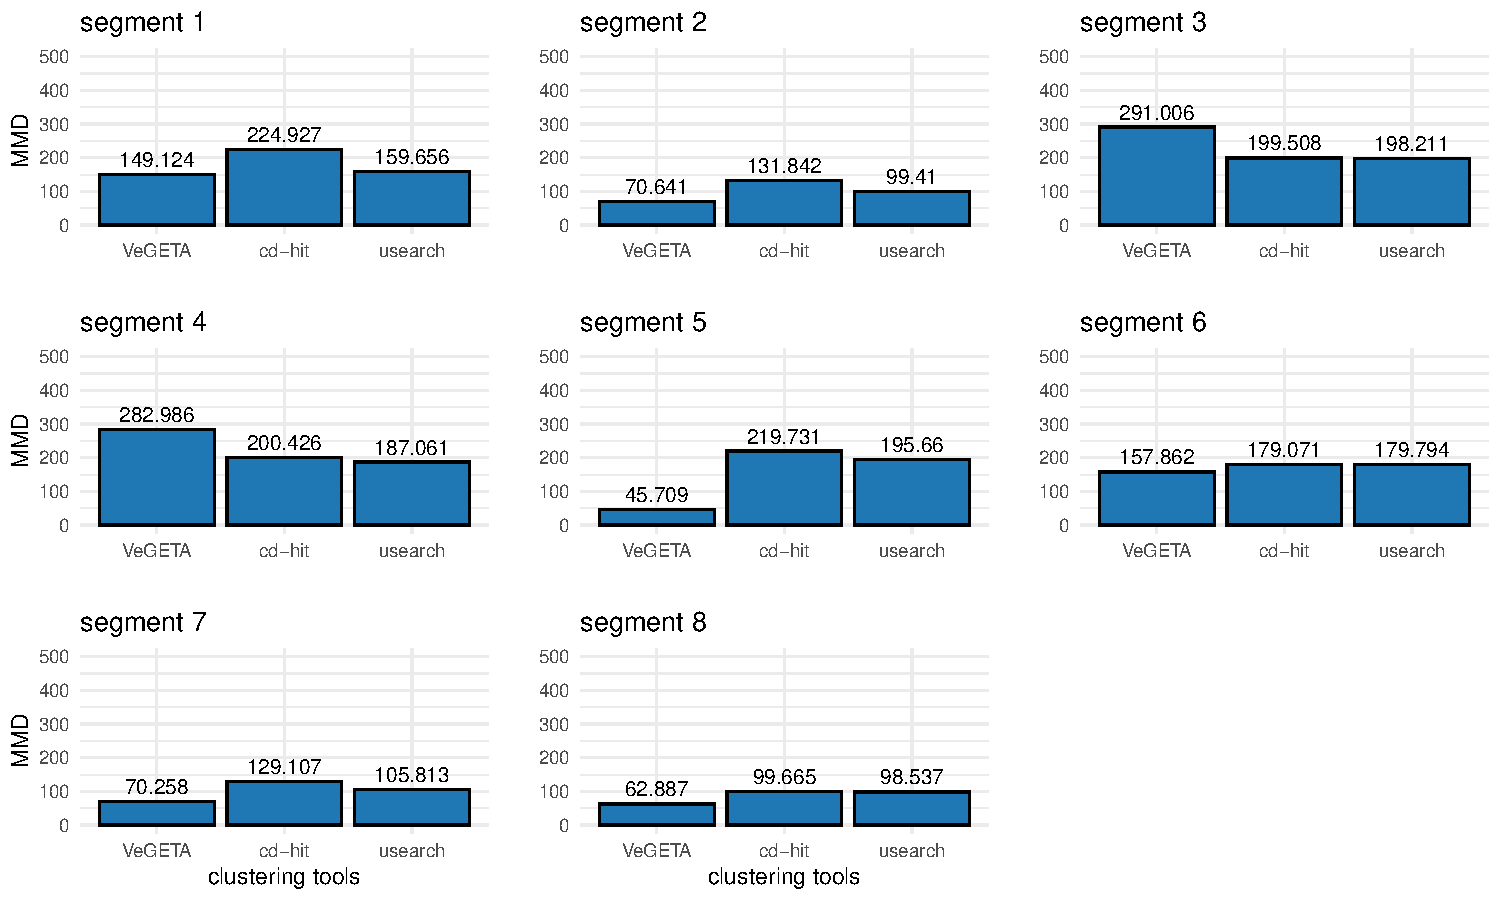
\includegraphics[width=\dimexpr\textwidth-2\fboxsep-2\fboxrule]{Figures/Seg_MMD.pdf}}
        \caption[Clustering quality of all segments measured with \gls{MMD}]{\textbf{Clustering quality of all segments measured with \gls{MMD}.} For all segments of \gls{IBV} the rating pipeline with \gls{MMD} as measurement was used to rate the quality of the clusters generated by CD-HIT, usearch and VeGETA. The distances are weighted by the cluster sizes generated by the tools.}
        \label{fig:3.8}
    \end{figure}
    
    \section{CD-HIT and usearch identity threshold comparison}
    
    Questioning the robustness of the rating related to the CD-HIT and usearch identity threshold settings, rating of segment five was repeated multiple times with different settings (\autoref{fig:3.9} and \autoref{fig:3.10}). While the clustering quality of both tools increased slightly with the use of the identity threshold 0.98, noticeable by a decrease of \gls{MED} and \gls{MMD}, there were no differences related to the ranking. With higher setting of 0.99, the number of single sequence clusters increased leading to an proportional increase of \gls{MED} and \gls{MMD}. By changing the threshold to 1.00, the clusters were mostly single sequence clusters leading to \gls{MED} higher than 50 and \gls{MMD} higher than 500. Repetition of comparison for the other segments may be necessary to find the optimum value for the identity threshold for usearch and CD-HIT yet the quality of VeGETA seems to be superior to the optimal CD-HIT and usearch settings. 
    
    \begin{figure}[!htb]
        \centering
        \fbox{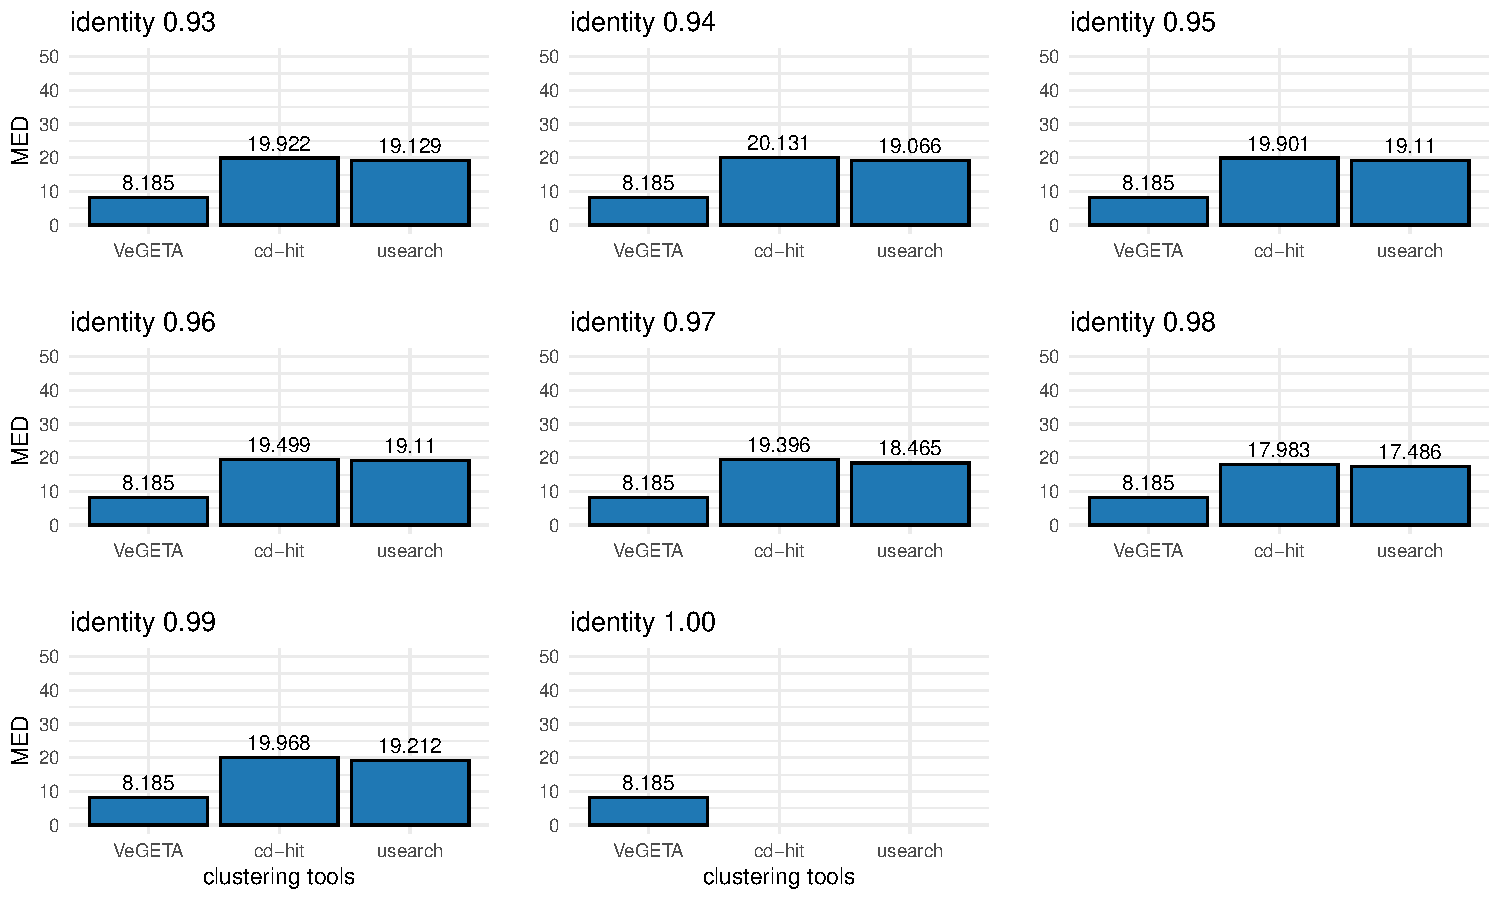
\includegraphics[width=\dimexpr\textwidth-2\fboxsep-2\fboxrule]{Figures/ID_MED.pdf}}
        \caption[Clustering quality of different thresholds measured with \gls{MED}]%
        {\textbf{Clustering quality of different thresholds measured with \gls{MED}.}%
        For segment five of \gls{IBV} and different sequence identity thresholds of CD-HIT and usearch, the rating pipeline with \gls{MED} as measurement was used to rate the quality of the clusters generated by CD-HIT, usearch and VeGETA. The distances are weighted by the cluster sizes generated by the tools.}
        \label{fig:3.9}
    \end{figure}
    
    \begin{figure}[!htb]
        \centering
        \fbox{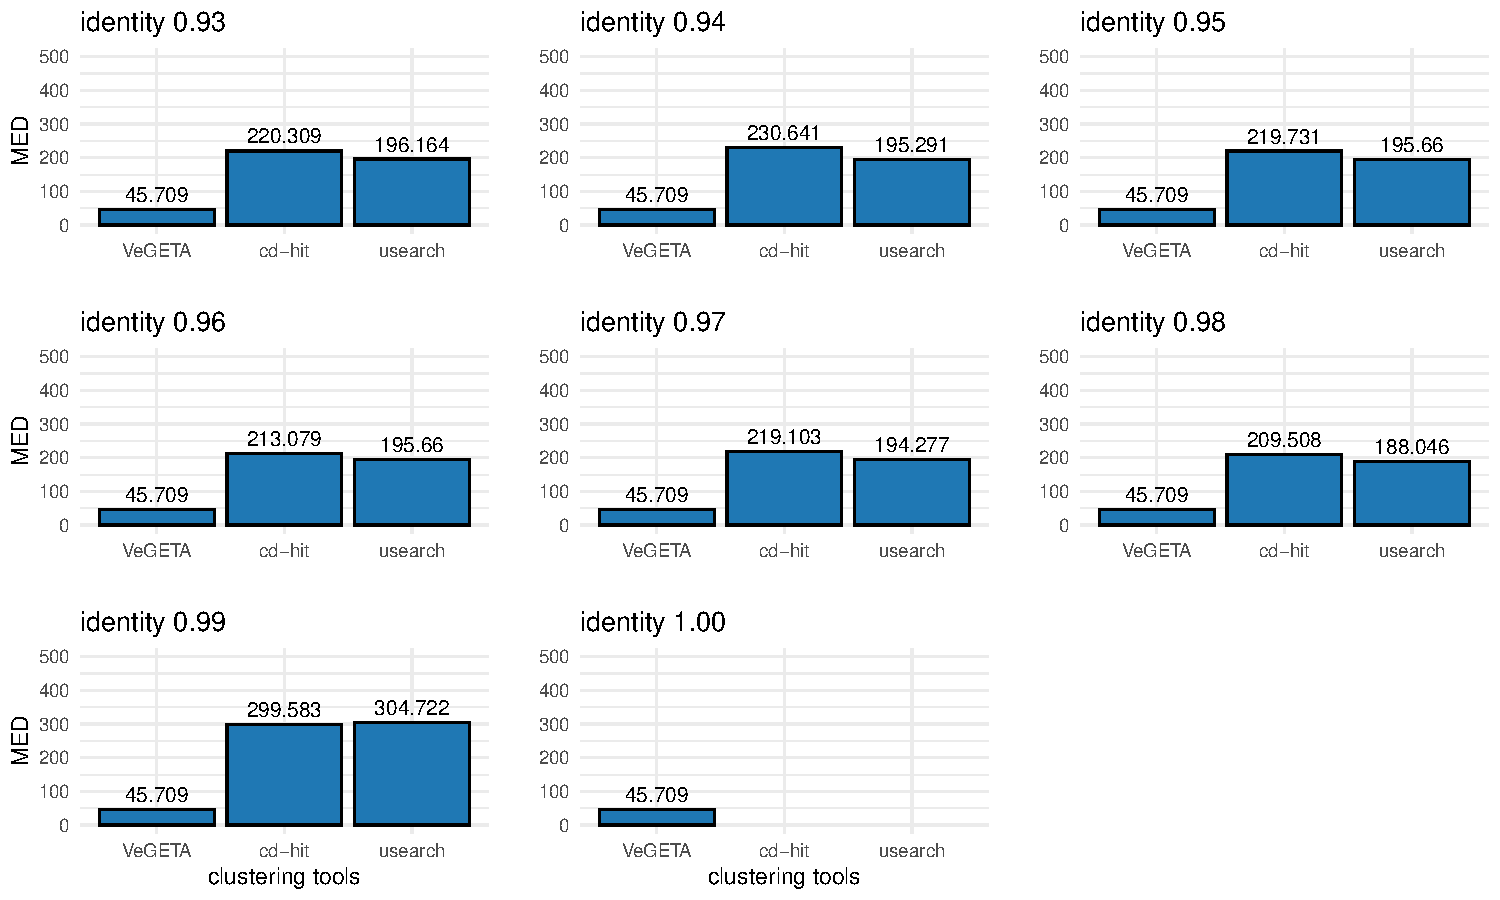
\includegraphics[width=\dimexpr\textwidth-2\fboxsep-2\fboxrule]{Figures/ID_MMD.pdf}}
        \caption[Clustering quality of different thresholds measured with \gls{MMD}]%
        {\textbf{Clustering quality of different thresholds measured with \gls{MMD}.}%
        For segment five of \gls{IBV} and different sequence identity thresholds of CD-HIT and usearch, the rating pipeline with \gls{MMD} as measurement was used to rate the quality of the clusters generated by CD-HIT, usearch and VeGETA. The distances are weighted by the cluster sizes generated by the tools.}
        \label{fig:3.10}
    \end{figure}
    
    \section{Clustering of \textit{Influenza B Virus} segment 8}\label{sec:3.1}
    
    \begin{table}[!htb]
        \centering
        \begin{tabu} to 1\textwidth{X[1.2,l]X[1,r]X[1,r]X[1,r]X[1.3,r]}
            \toprule
    		\textbf{tool} & \ltab\textbf{cluster} & \ltab\textbf{MED} & \ltab\textbf{MMD} & \ltab\textbf{cluster size $\bm{m}$}\\
    		\midrule
    		CD-HIT&0&15.056& 99.688 &488\\
            CD-HIT&1&15.036& 98.727 &12\\
            usearch&0&14.886& 98.557 &432\\
            usearch&1&14.702& 98.413 &68\\
            VeGETA&0&9.883& 41.719 &18\\
            VeGETA&1&10.415& 49.856 &18\\
            VeGETA&2&8.100& 37.806 &34\\
            VeGETA&3&8.076& 35.103 &70\\
            VeGETA&4&6.445& 28.145 &11\\
            VeGETA&5&10.861& 58.606 &126\\
            VeGETA&6&12.362& 65.820 &25\\
            VeGETA&7&15.873& 102.860 &106\\
            VeGETA&8&5.663& 14.156 &10\\
            VeGETA&9&12.628& 69.896 &73\\
    		\bottomrule
    	\end{tabu}
    	\caption[\gls{MED} of \gls{IBV} segment eight clusters]{\textbf{\gls{MED} of \gls{IBV} segment eight clusters.} The \gls{MED} and \gls{MMD} for all the clusters generated by the used tools with their related cluster size.}
        \label{tab:3.1}
    \end{table}
     
    \begin{figure}[!htb]
        \centering
        \fbox{\includegraphics[width=\dimexpr\textwidth-2\fboxsep-2\fboxrule]{Figures/veg_letter.pdf}}
        \caption[Radial cladogram representing VeGETA clustering]{\textbf{Radial cladogram representing VeGETA clustering.} The evolutionary tree of the used segment eight sequences of \gls{IBV}, created by RAxML and colored related to the clusters created by VeGETA. For better comparison the areas A and B were cropped and enlarged in \autoref{fig:3.4}.}
        \label{fig:3.3}
    \end{figure}
    
    \begin{figure}[!htb]
        \centering
        \subcaptionbox{Top area}[.475\textwidth]{\fbox{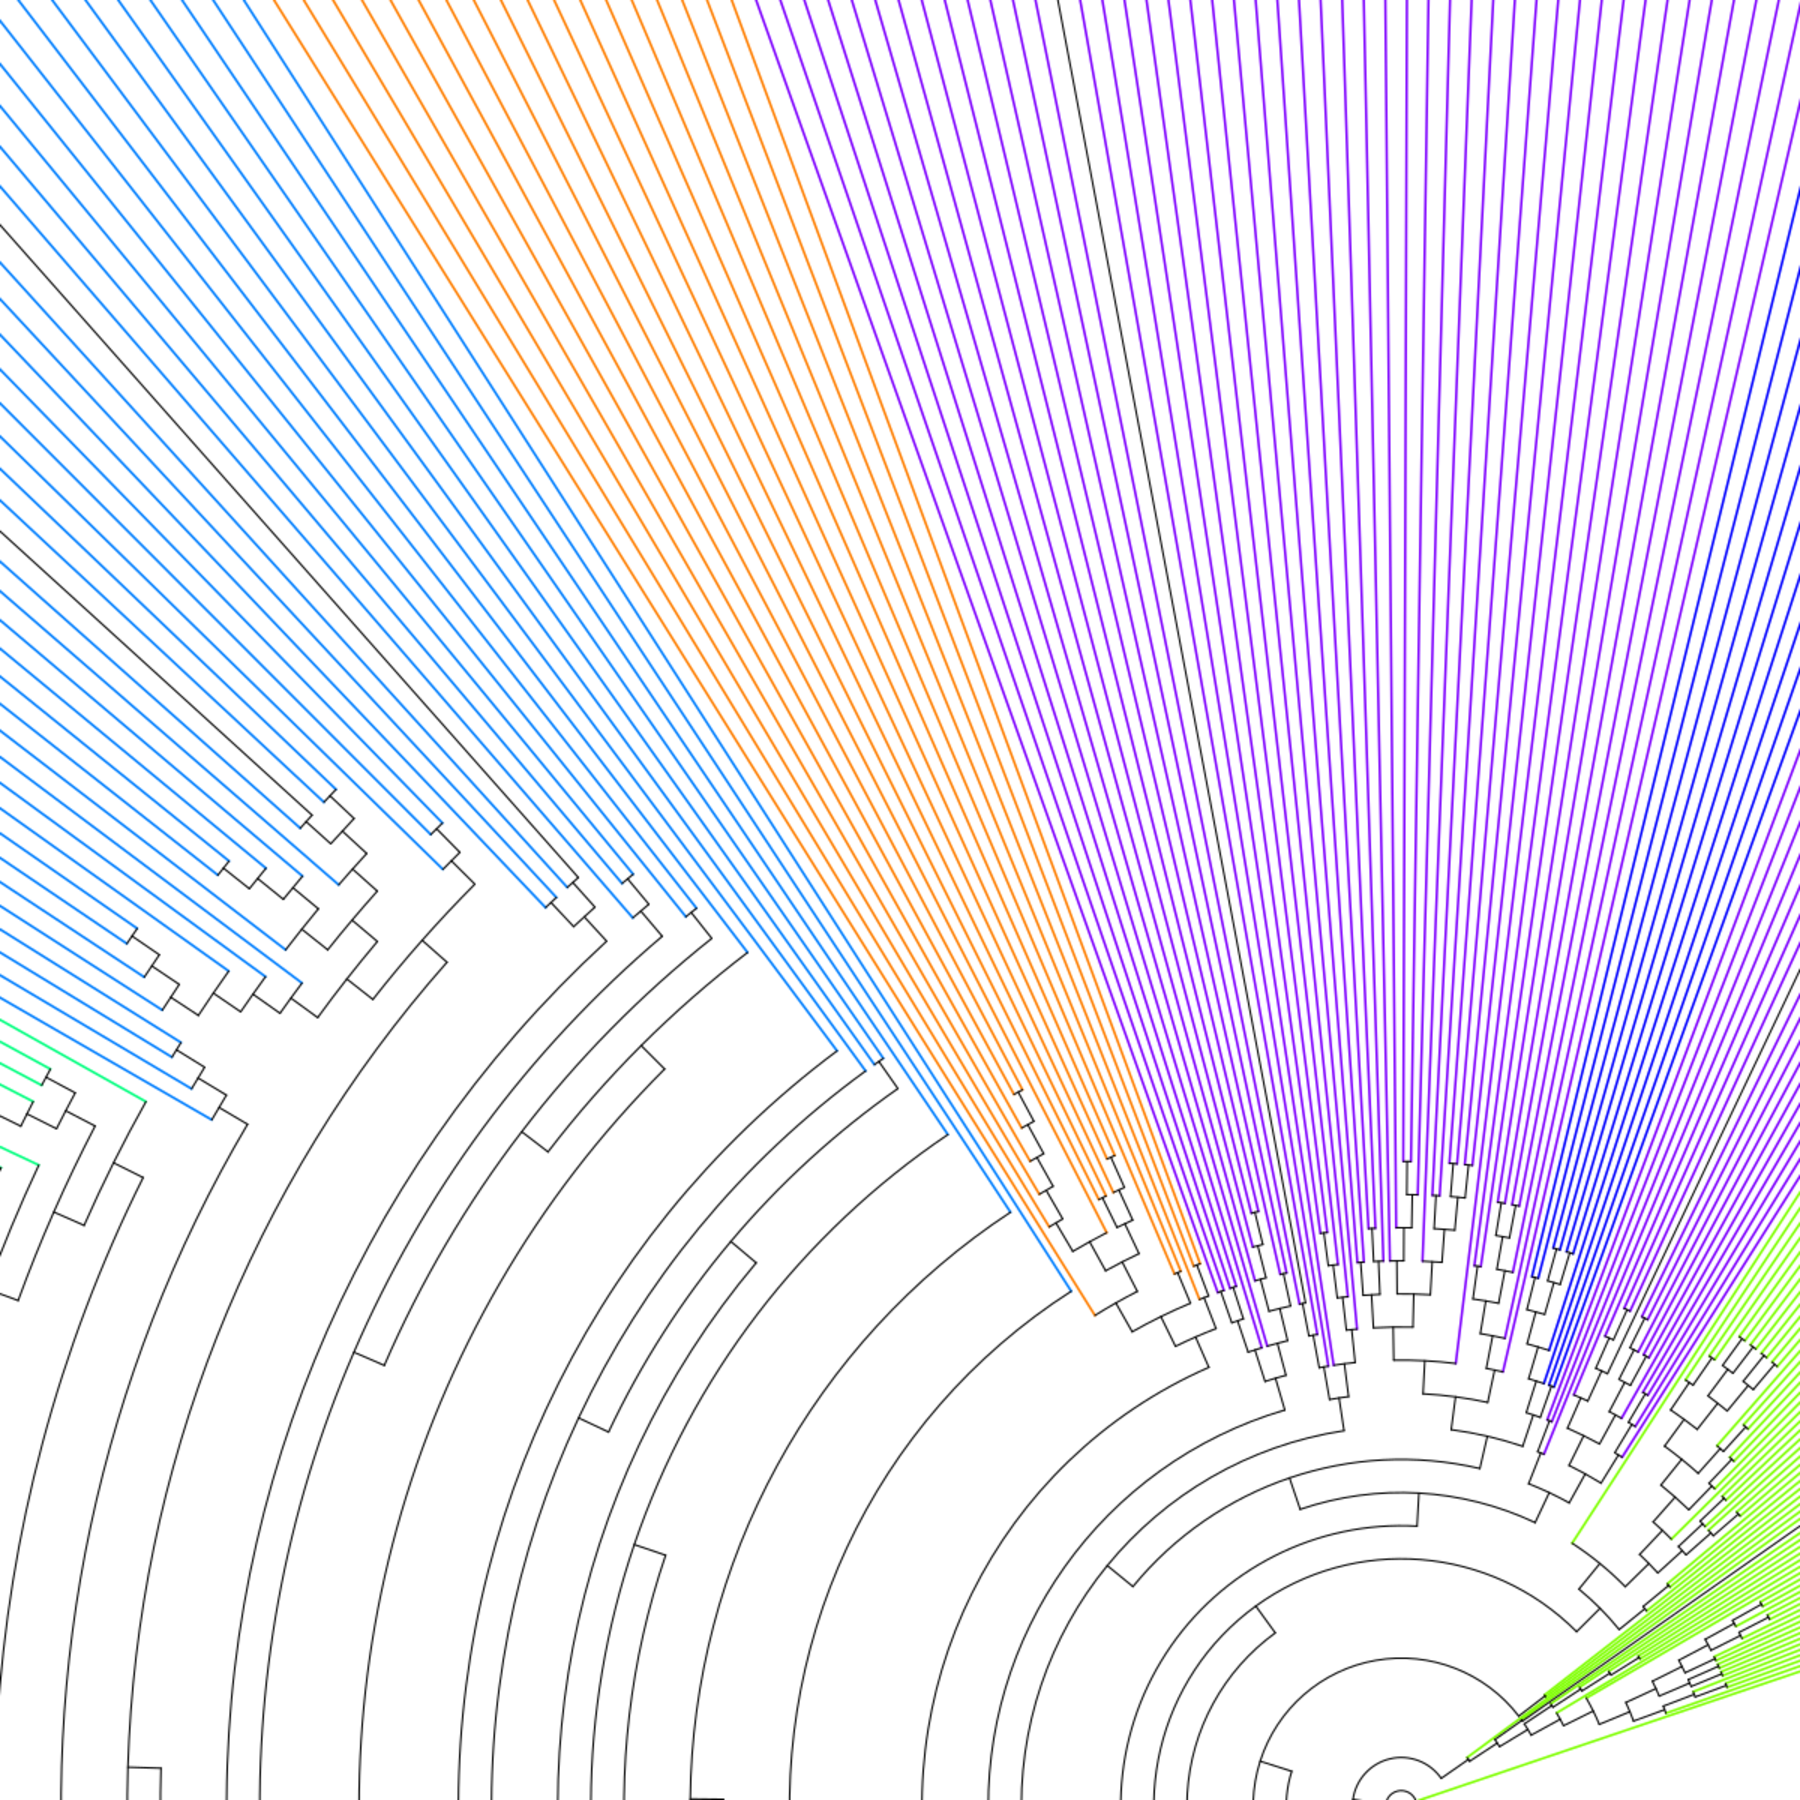
\includegraphics[width=.475\textwidth-2\fboxsep-2\fboxrule]{Figures/veg_left.pdf}}}\hfill 
        \subcaptionbox{Bottom area}[.475\textwidth]{\fbox{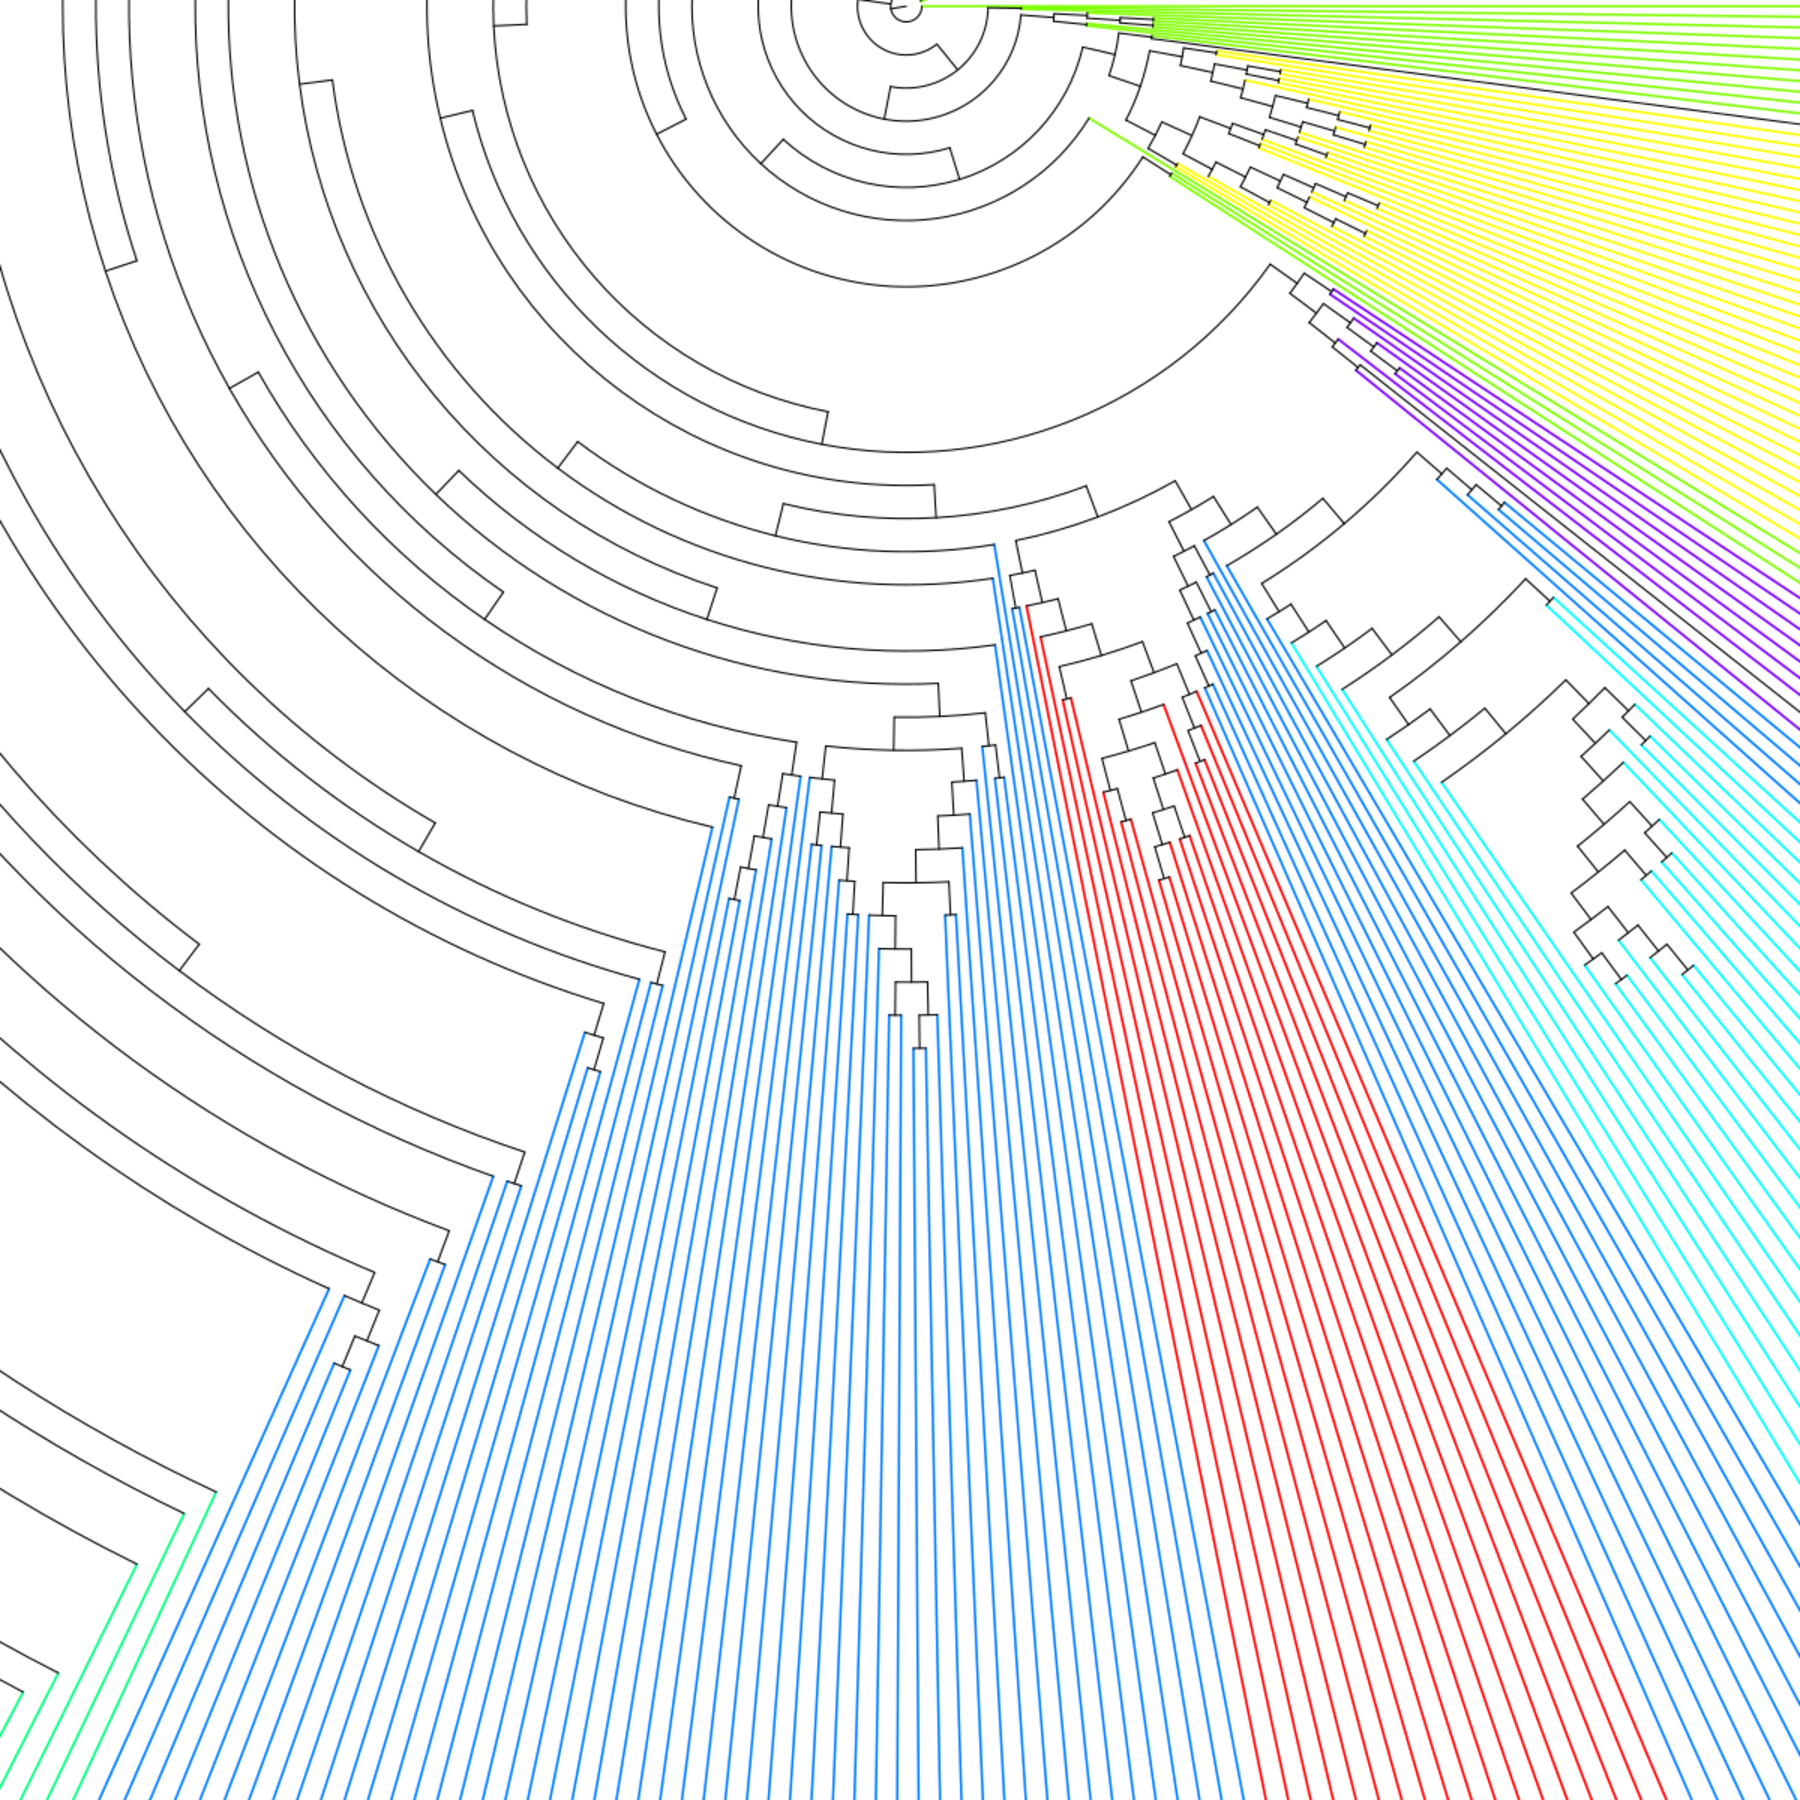
\includegraphics[width=.475\textwidth-2\fboxsep-2\fboxrule]{Figures/veg_down.pdf}}}
        \caption[Focus on VeGETA colored cladogram \autoref{fig:3.3}]{\textbf{Focus on VeGETA colored cladogram \autoref{fig:3.3}.} Enlargement of area A and B of \autoref{fig:3.3} for better comparison of the clustering behavior of VeGETA. The coloring resemble the created clusters.}
        \label{fig:3.4}
    \end{figure}
    
    After elaboration of a reliable approach to rank clustering tools, as well as rate their clustering quality, the used tool VeGETA was compared to sequence identity based tools usearch and CD-HIT. For a quick overview, a radial cladogram of the used sequences was build and colored based on the clustering of VeGETA (\autoref{fig:3.3}) \autocite{vegeta}. By focusing on the marked windows in \autoref{fig:3.4}, the high number of clusters calculated by VeGETA became visible. Comparison with the same windows for the radial cladograms of CD-HIT \autoref{fig:3.5} and usearch \autoref{fig:3.6}, indicated these big differences in the clustering algorithms compared to VeGETA. This was leveraged by \autoref{tab:3.1}. While usearch and CD-HIT only calculated two clusters each, one big cluster of 488 sequences in CD-HIT and 432 sequences in usearch as well as a small one with 12 in CD-HIT and 68 in usearch, VeGETA split the sequences in 10 clusters.
    
    \begin{figure}[!htb]
        \centering
        \subcaptionbox{Top area}[.475\textwidth]{\fbox{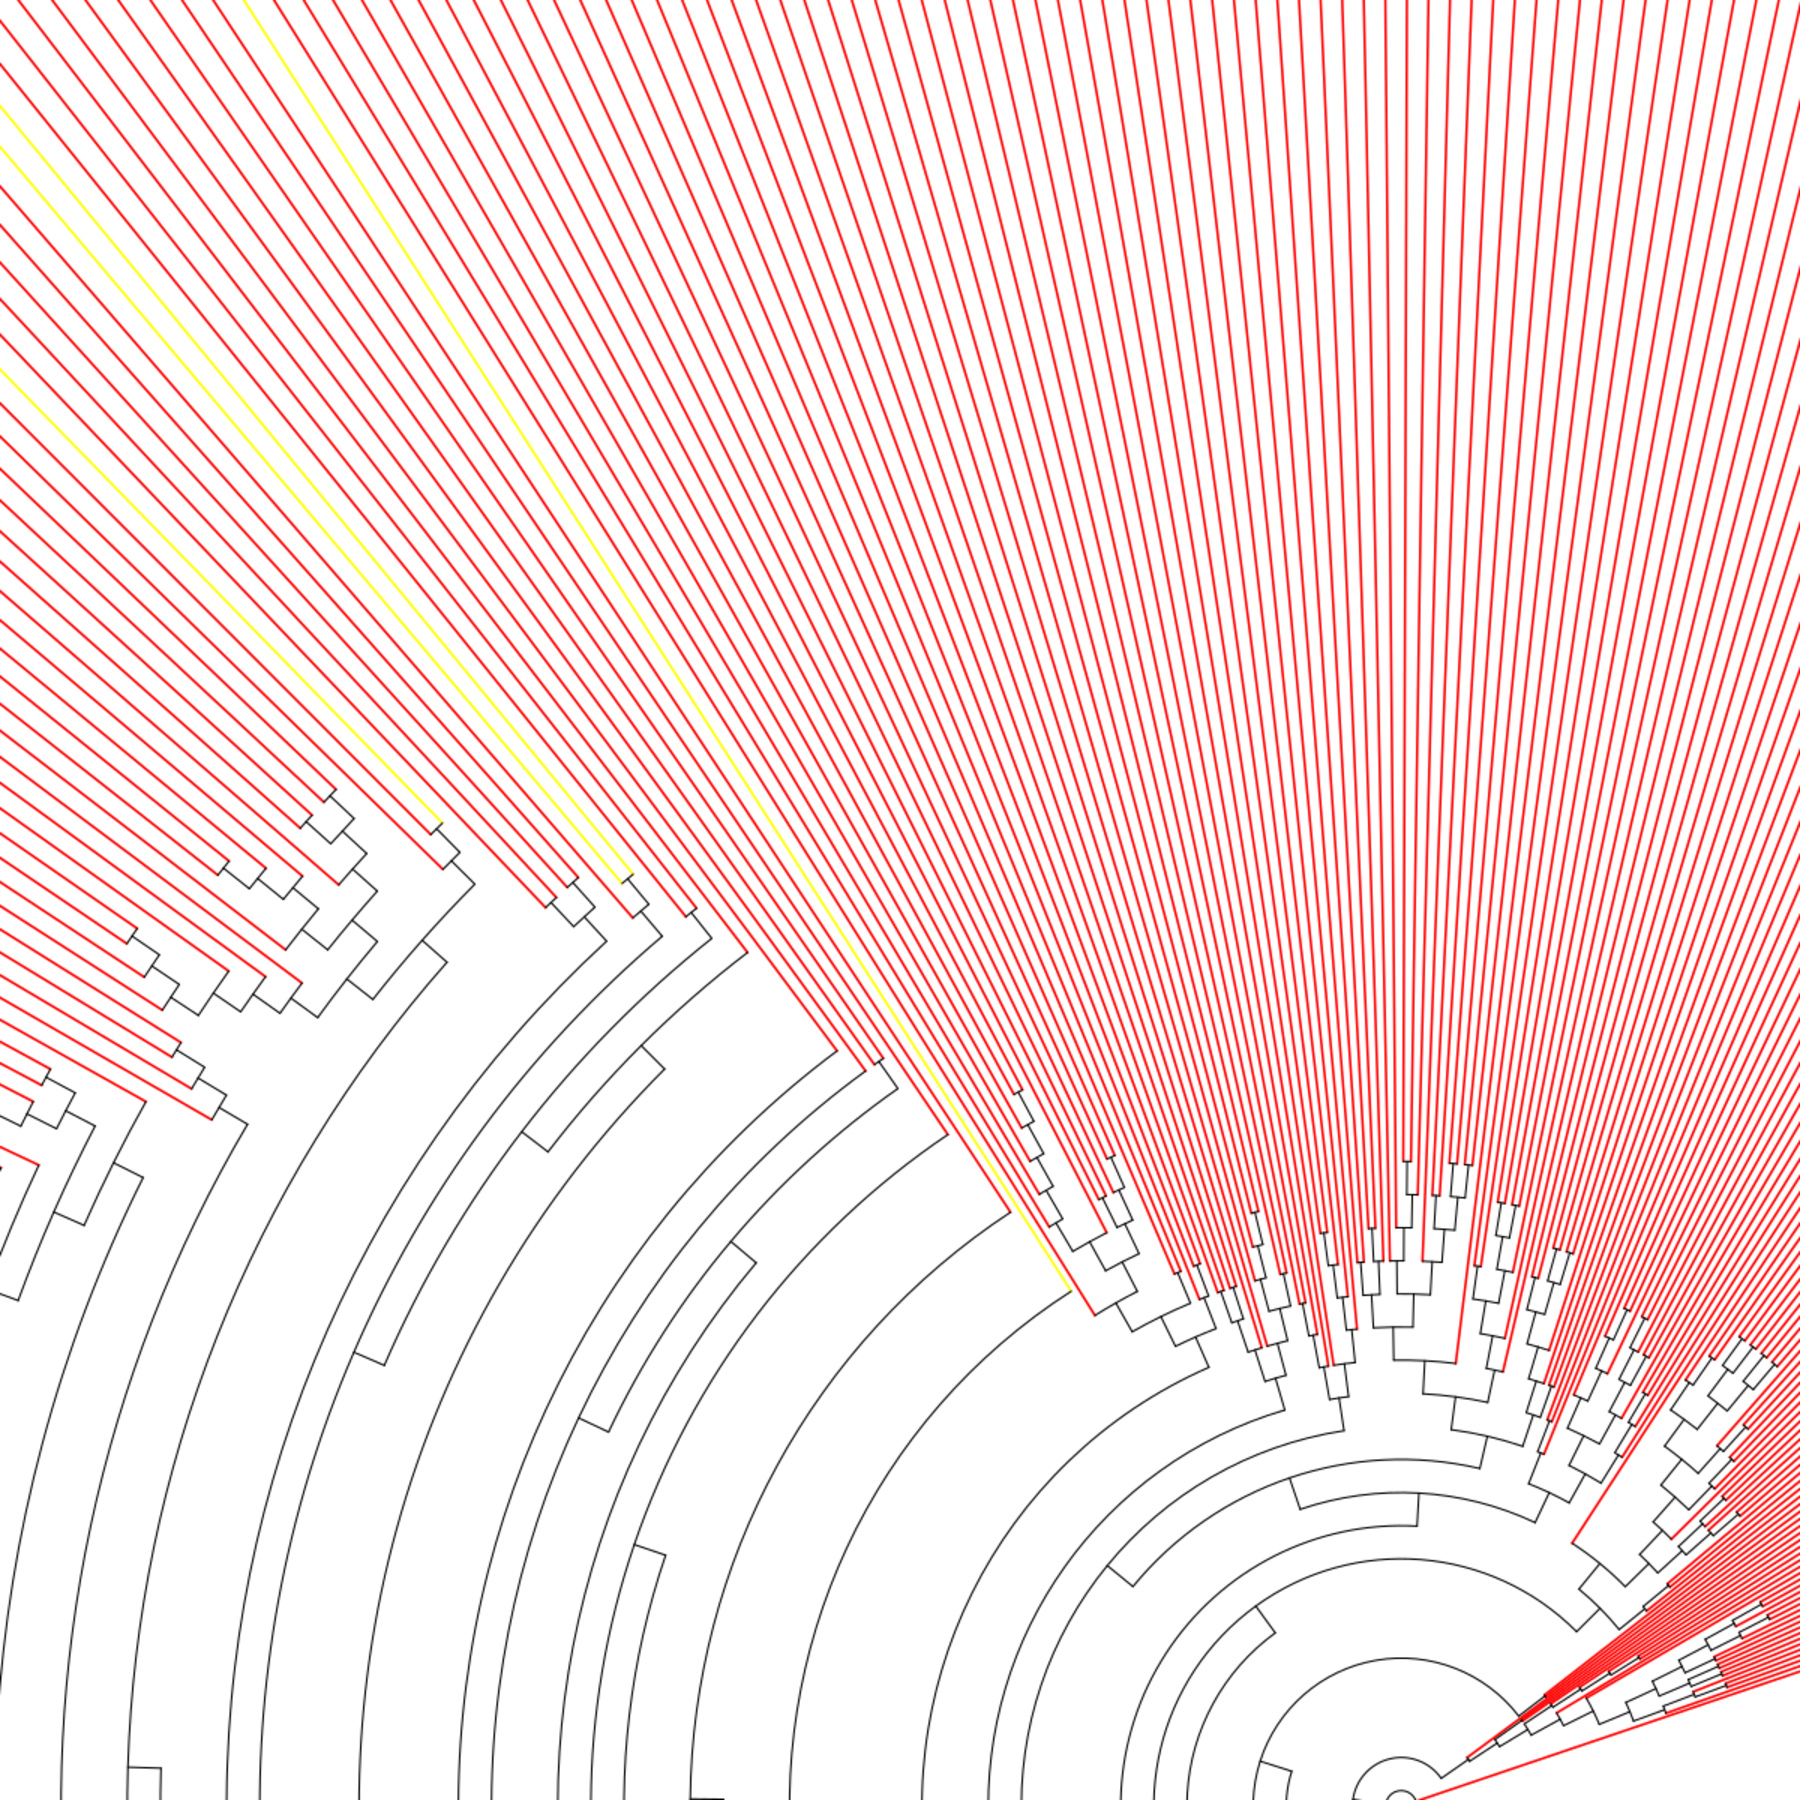
\includegraphics[width=.475\textwidth-2\fboxsep-2\fboxrule]{Figures/cdh_left.pdf}}}\hfill 
        \subcaptionbox{Bottom area}[.475\textwidth]{\fbox{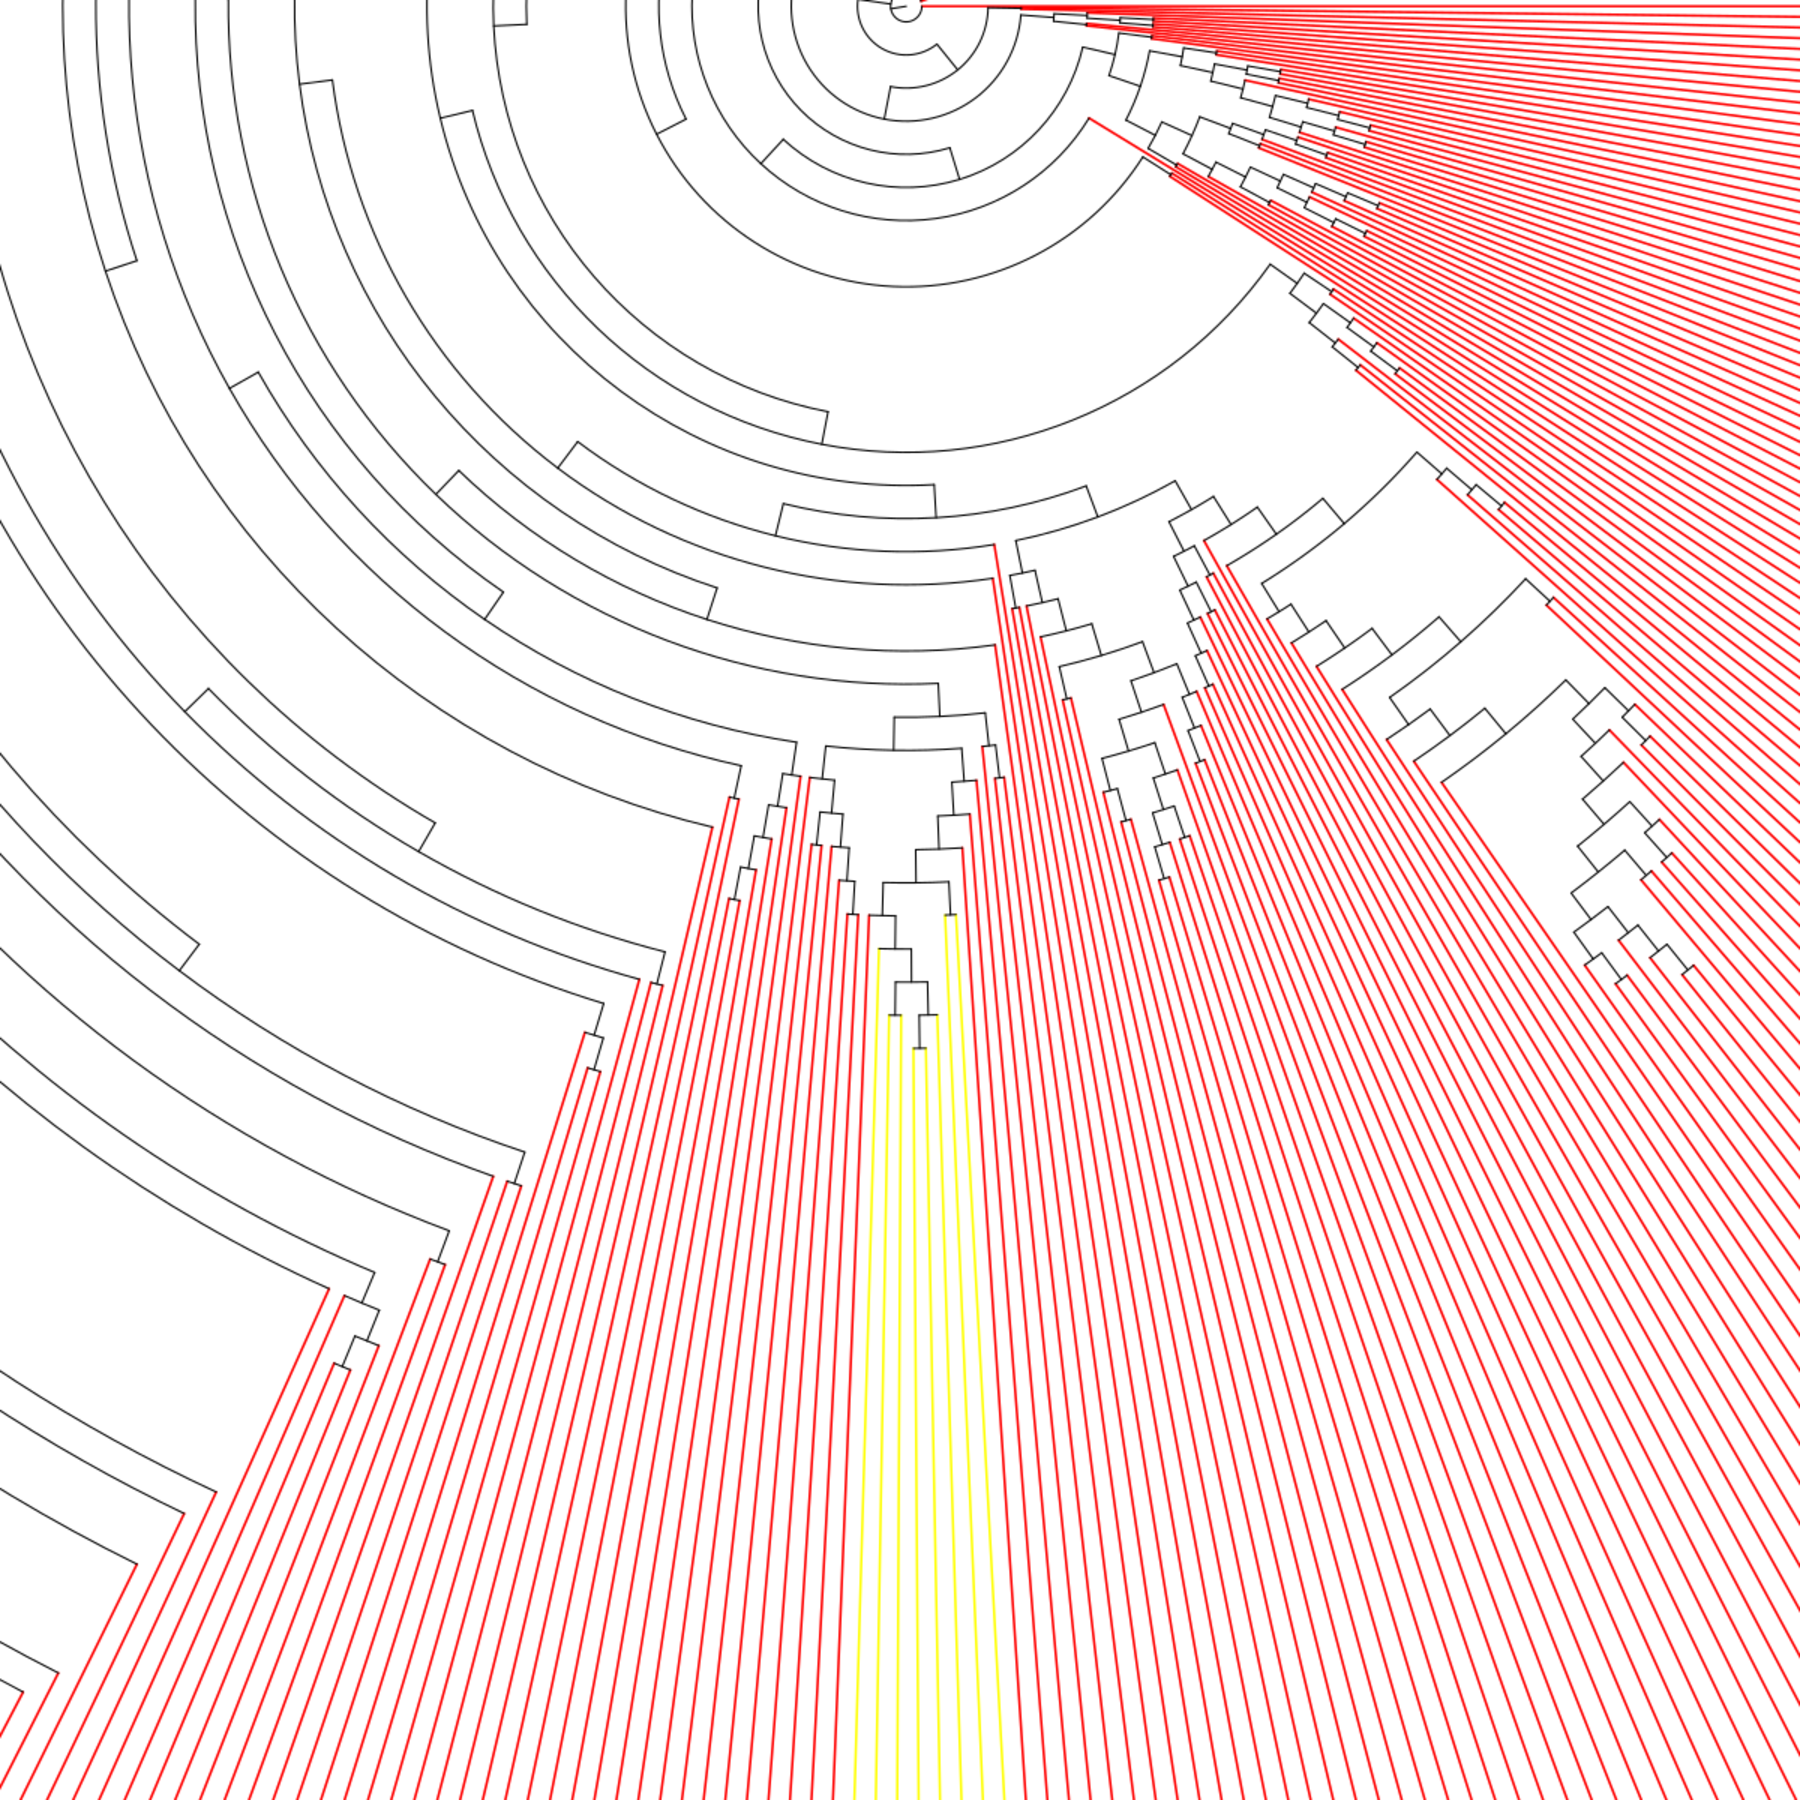
\includegraphics[width=.475\textwidth-2\fboxsep-2\fboxrule]{Figures/cdh_down.pdf}}}
        \caption[Focus on CD-HIT colored cladogram \autoref{fig:A.1}]{\textbf{Focus on CD-HIT colored cladogram \autoref{fig:A.1}.} Enlargement of area A and B of \autoref{fig:A.1} for better comparison of the clustering behavior of CD-HIT. The coloring resemble the created clusters.}
        \label{fig:3.5}
    \end{figure}
    
    Precise inspection of the \gls{MED} per cluster in \autoref{tab:3.1} showed smaller distances in nine of ten clusters, calculated by VeGETA, than in the two clusters from usearch and CD-HIT. The summary of these results in \autoref{tab:3.1} indicated the same conclusion. While the cluster with the biggest mean of \gls{MED} in VeGETA with 15.873 was only slightly bigger than the clusters with the biggest mean of \gls{MED} in CD-HIT (15.056) and usearch (14.886), there were even plenty of better ones in VeGETA. This concluded to the fact, that even with a sequence based rating approach, like the one proposed in this project, the new tool VeGETA seemed to create more compact clusters. This assumption was supported by the fact, that VeGETA had the smallest \gls{MED} values, in the visualization of the \gls{MED} for all segments of \gls{IBV} in \autoref{fig:3.7}, stating the compactness of the created clusters.
    
    \begin{figure}[!htb]
        \centering
        \subcaptionbox{Top area}[.475\textwidth]{\fbox{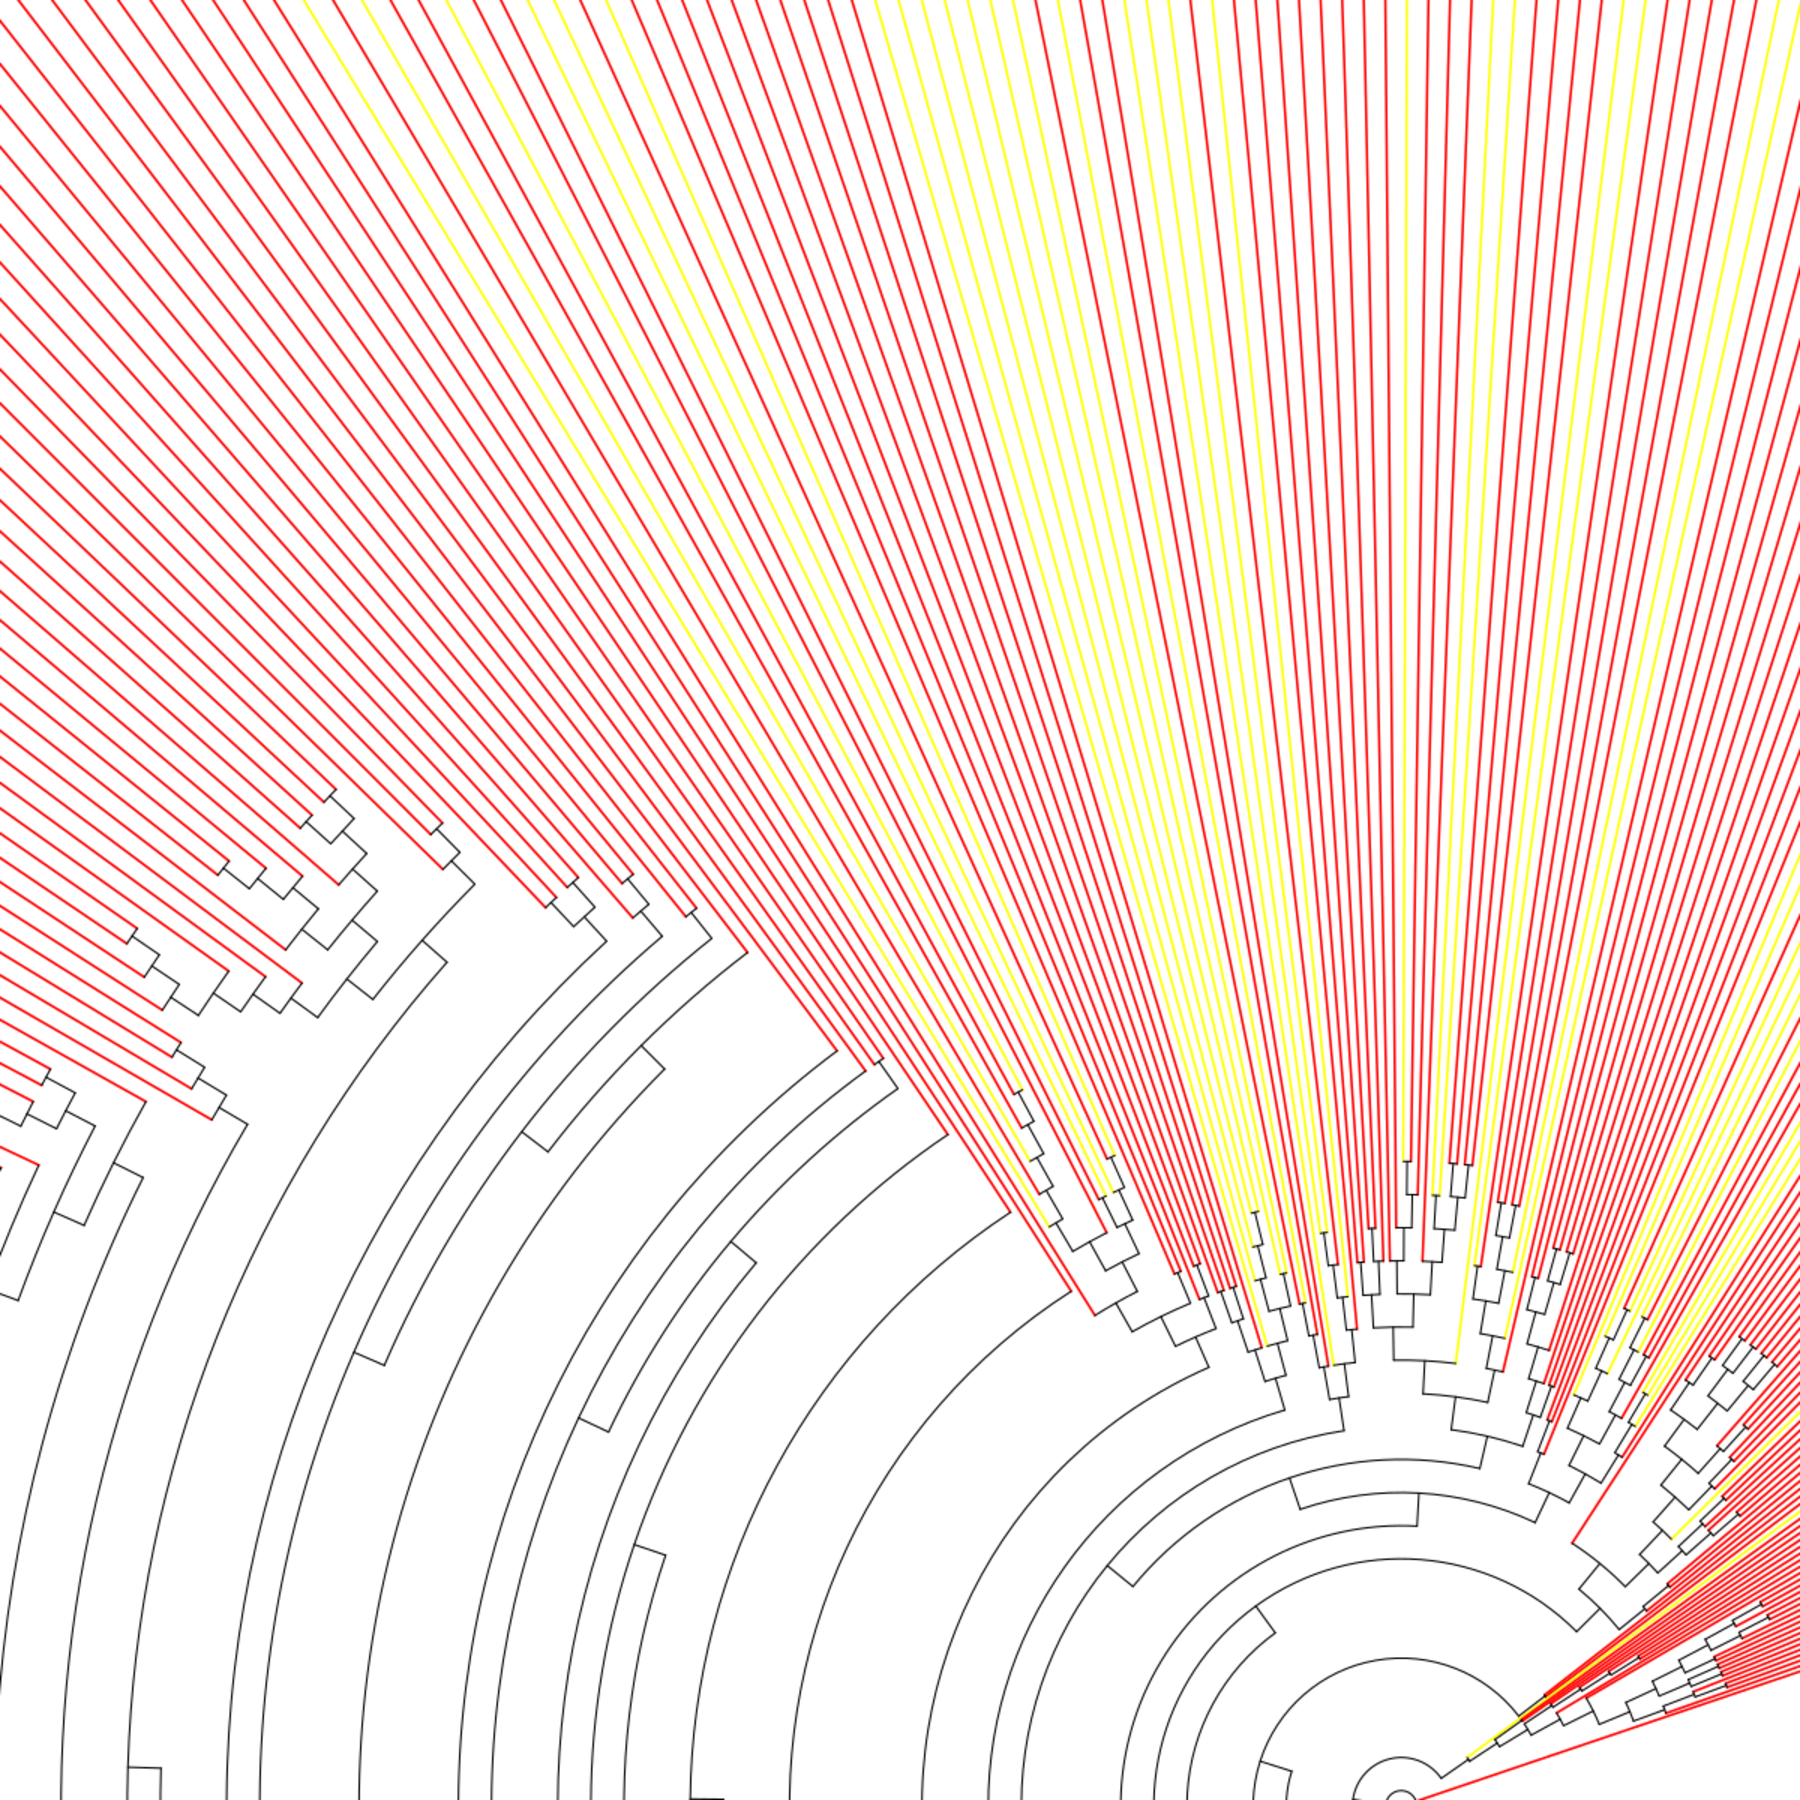
\includegraphics[width=.475\textwidth-2\fboxsep-2\fboxrule]{Figures/ucl_left.pdf}}}\hfill 
        \subcaptionbox{Bottom area}[.475\textwidth]{\fbox{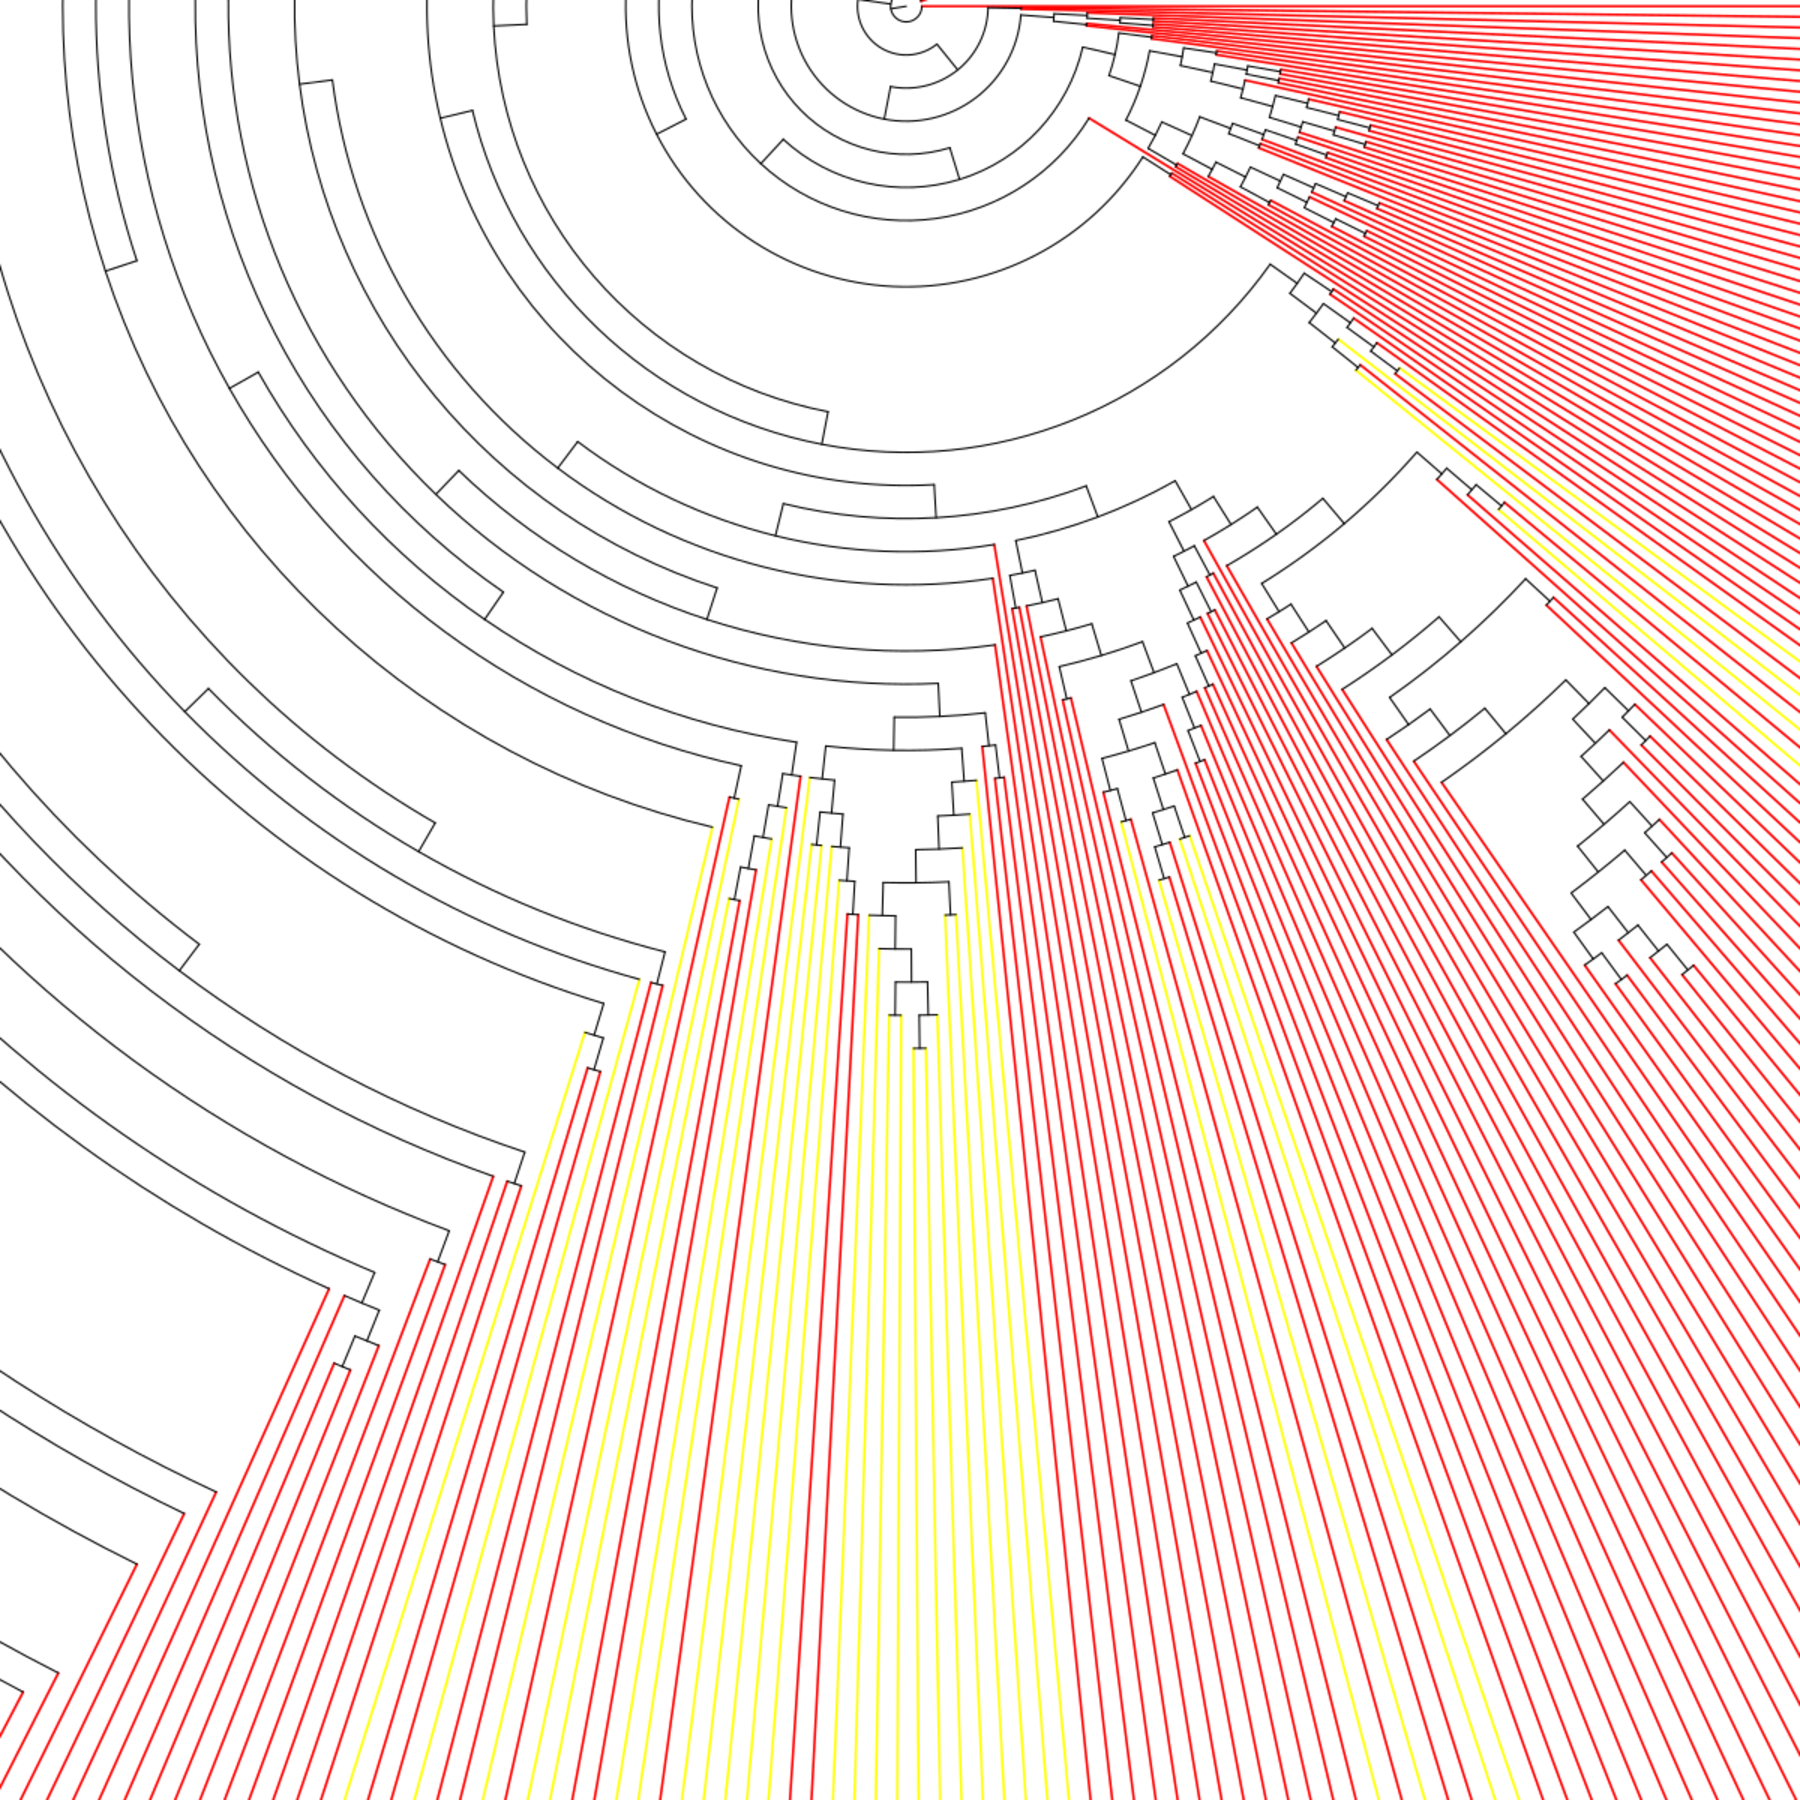
\includegraphics[width=.475\textwidth-2\fboxsep-2\fboxrule]{Figures/ucl_down.pdf}}}
        \caption[Focus on usearch colored cladogram \autoref{fig:A.2}]{\textbf{Focus on usearch colored cladogram \autoref{fig:A.2}.} Enlargement of area A and B of \autoref{fig:A.1} for better comparison of the clustering behavior of usearch. The coloring resemble the created clusters.}
        \label{fig:3.6}
    \end{figure}

    This result was still obtained by using a sequence identity based rating approach on different clustering methods. While even changing the identity threshold of CD-HIT and usearch did not seem to change the results in any way, it might still be necessary to validate these result with a second cluster rating approach based on evolutionary distance. Repeating the pipeline with an optimal identity threshold for usearch and CD-HIT may still be important for more confident ranking. Nevertheless, the clustering of VeGETA was distinguished as most compact and best fitting for \gls{IBV} clustering by this version of cluster quality rating pipeline.
    
    \section{Secondary structures of \textit{Influenza B Virus} segment 8}
    
    \begin{figure}[!htb]
        \centering
        \fbox{
\includegraphics[width=0.6\textwidth-2\fboxsep-2\fboxrule]{Figures/structure.png}}
        \caption[Hairpin structure 5'-splice site]{\textbf{Hairpin structure 5'-splice site.} Recreation of the hairpin structure in segment eight of \gls{IBV}, proposed by \textcite{structure_BC} with a \gls{msa} from the segments representatives, found by VeGETA.}
        \label{fig:3.11}
    \end{figure}
    
    \begin{figure}[!htb]
        \centering
        \fbox{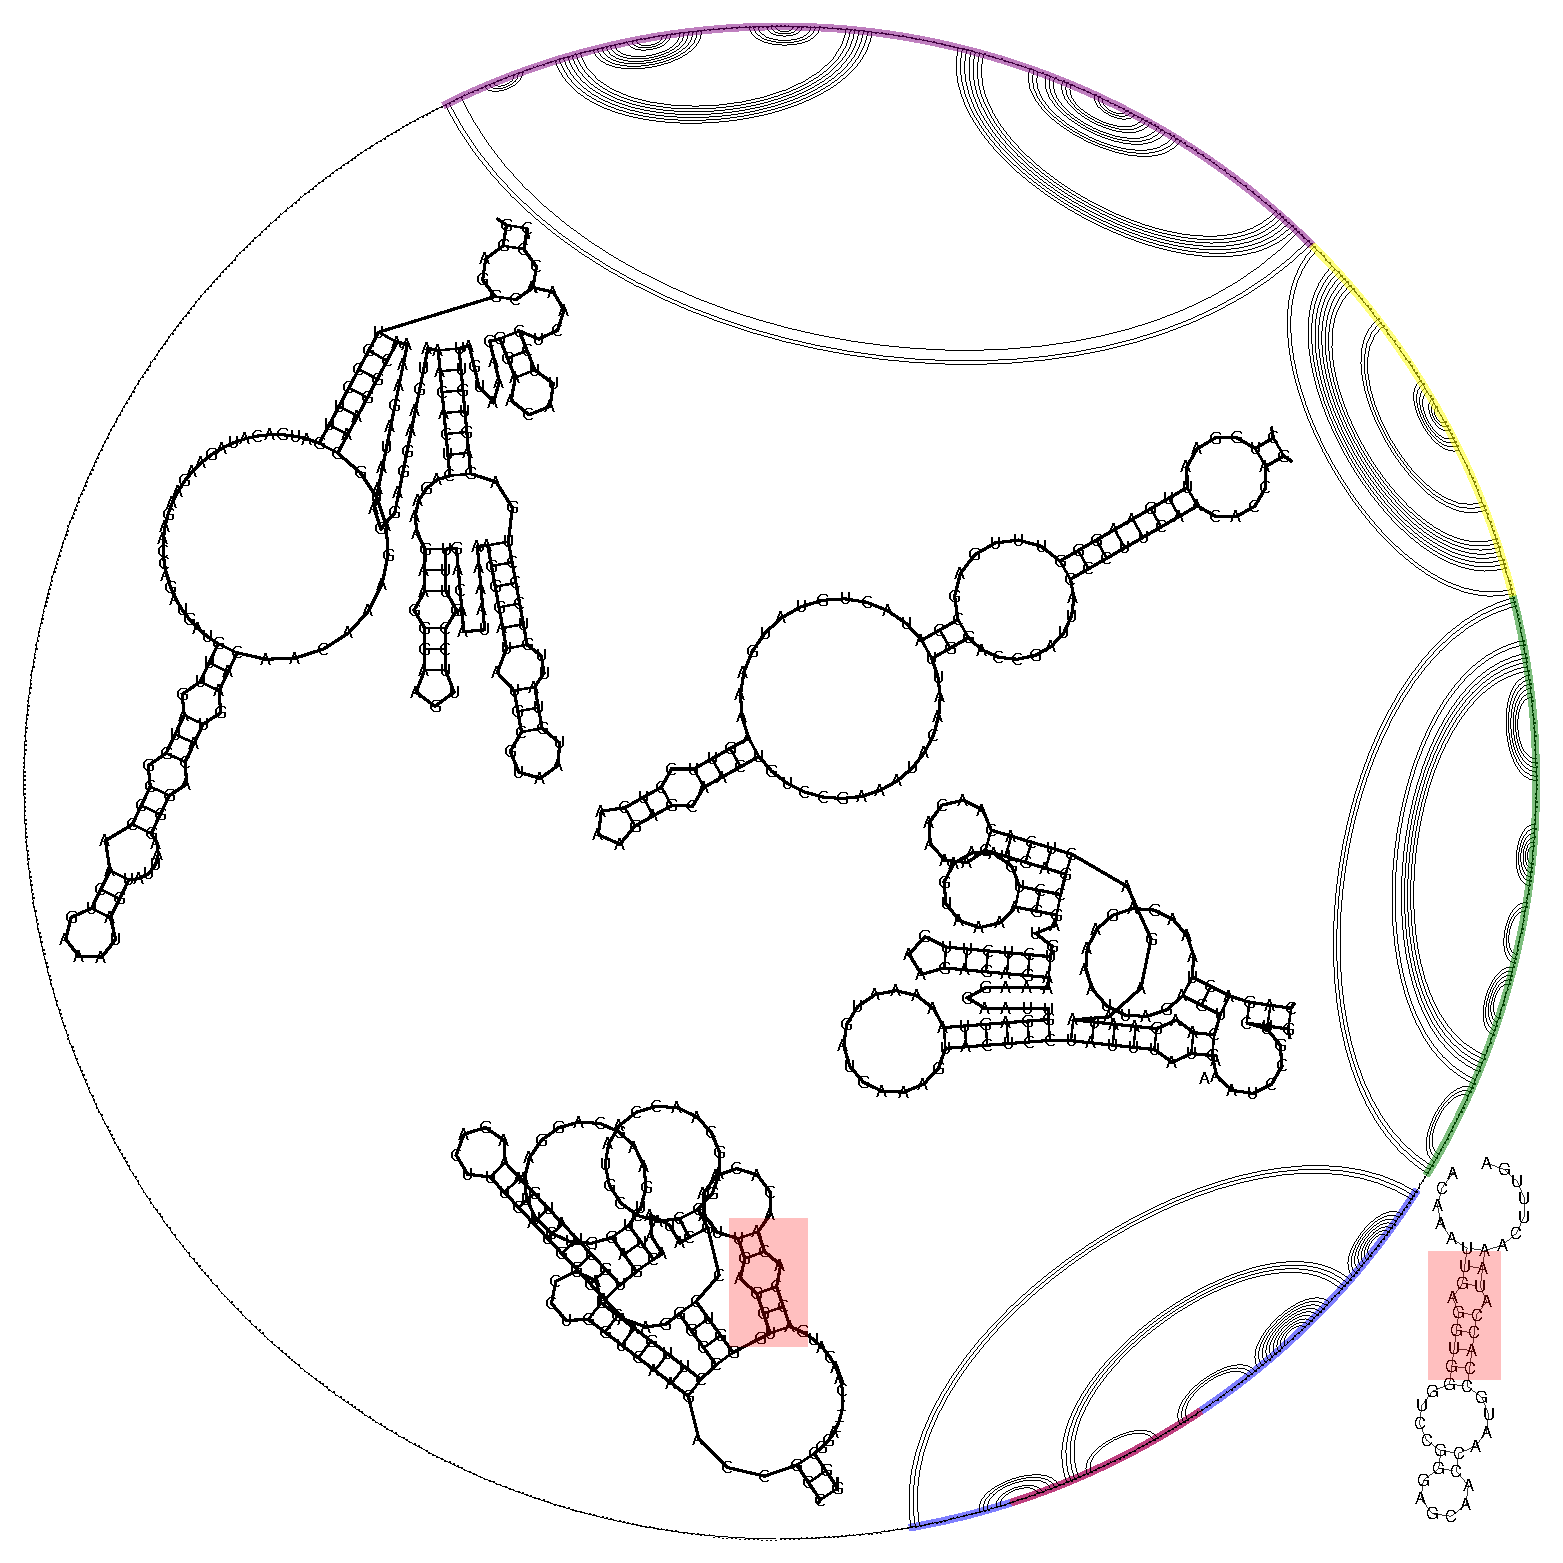
\includegraphics[width=\dimexpr\textwidth-2\fboxsep-2\fboxrule]{Figures/08_colored.pdf}}
        \caption[Secondary structure of \gls{IBV} segment seven calculated by VeGETA]{\textbf{Secondary structure of \gls{IBV} segment eight calculated by VeGETA.} All the secondary structure areas of the segment eight sequences of \gls{IBV} found by VeGETA, with their related folded structures for better visualization.}
        \label{fig:3.12}
    \end{figure}
    
    \begin{figure}[!htb]
        \centering
        \fbox{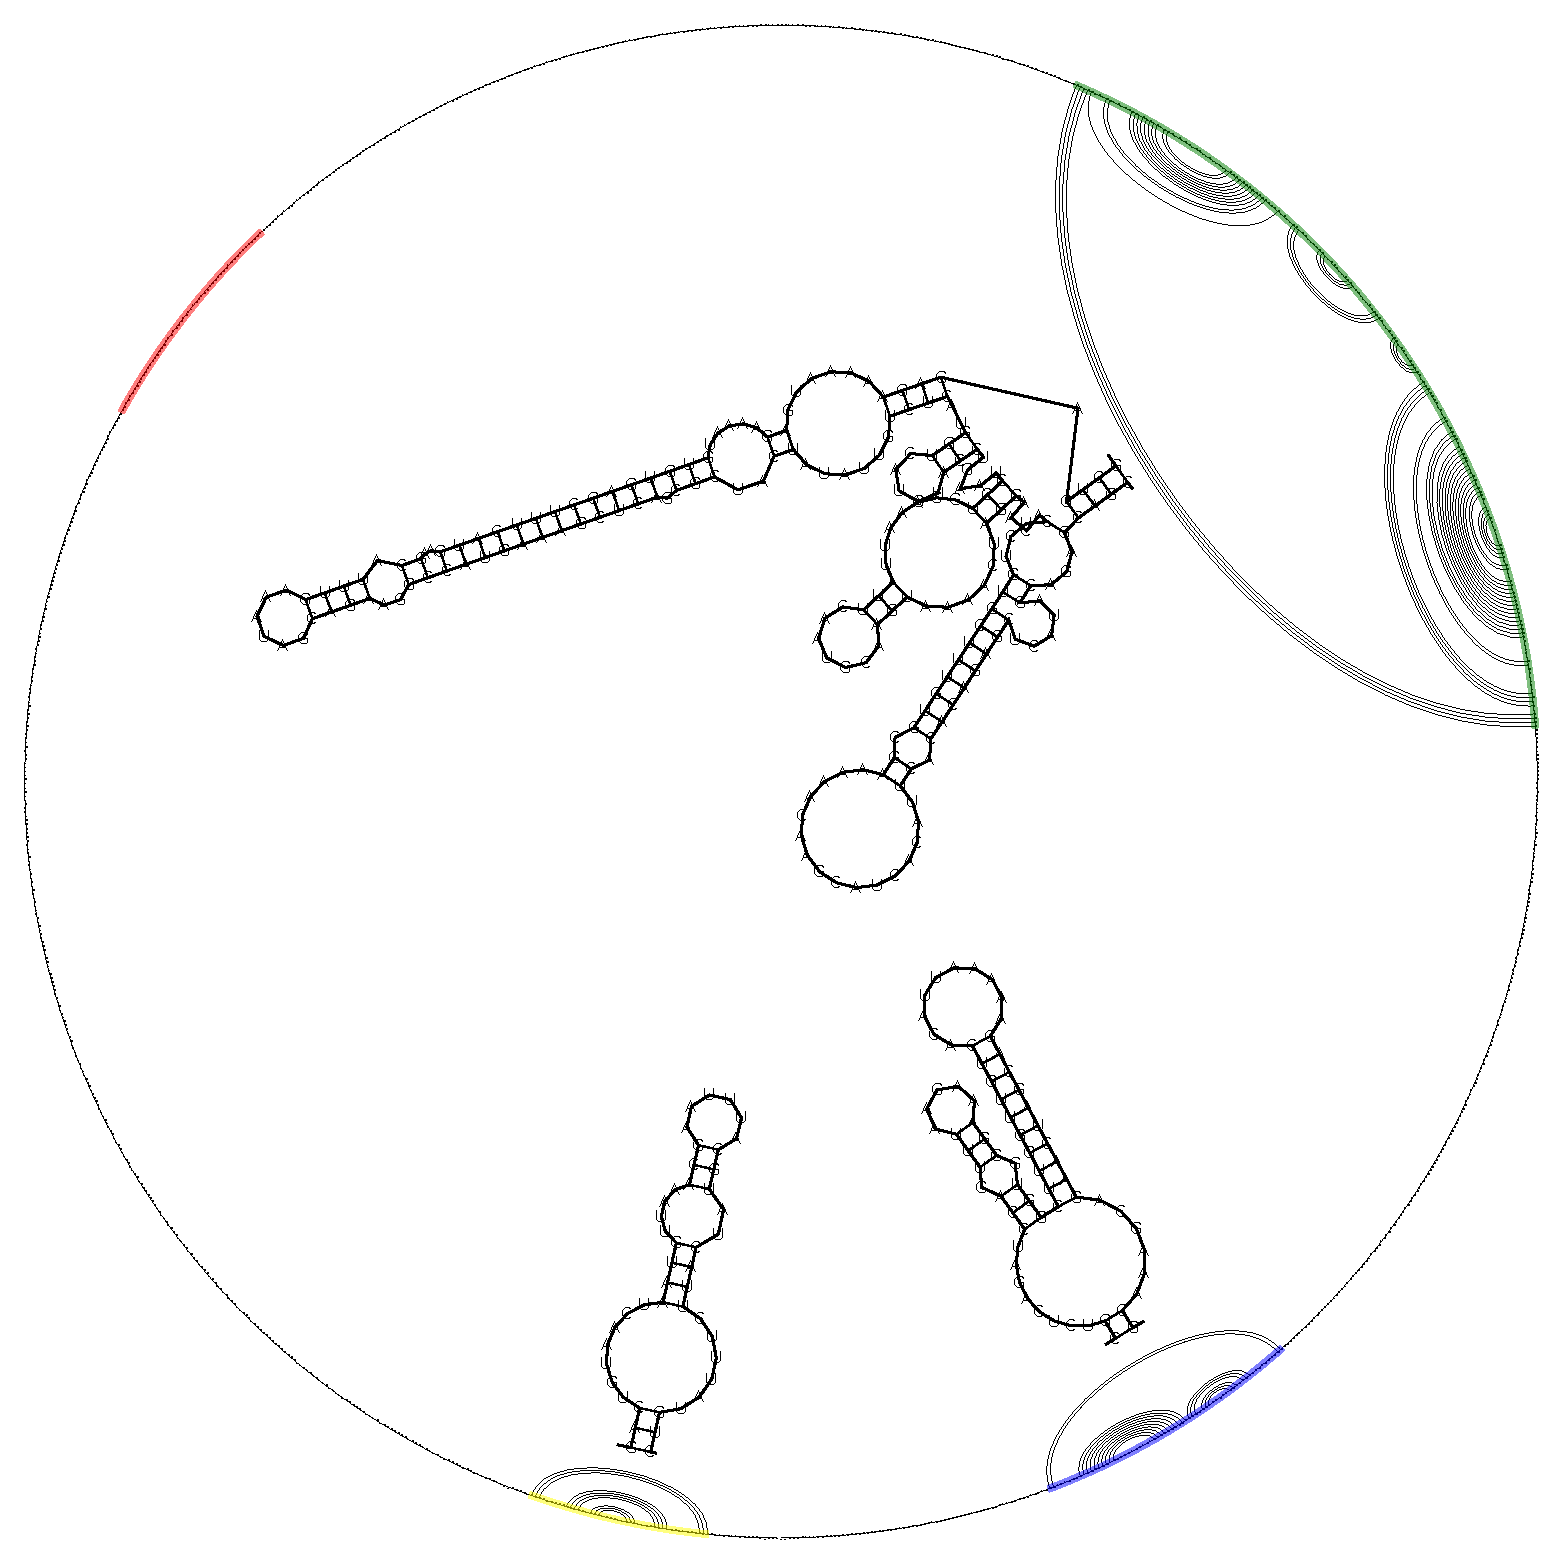
\includegraphics[width=\dimexpr\textwidth-2\fboxsep-2\fboxrule]{Figures/07_colored.pdf}}
        \caption[Secondary structure calculated by VeGETA]{\textbf{Secondary structure of \gls{IBV} segment seven calculated by VeGETA.} All the secondary structure areas of the segment seven sequences of \gls{IBV} found by VeGETA, with their related folded structures for better visualization.}
        \label{fig:3.13}
    \end{figure}
    
    The overall secondary structure calculated by VeGETA from the subset of \glspl{IBV} segment eight and visualized by RNAplot showed many structure elements (areas colored in purple, yellow, green and blue) (\autoref{fig:3.12}). While most structures could not be validated,
    %The top left green square represents the start of the \gls{ORF} reading in the direction of the black arrow. The green square on the right represents the stop codon and therefore the end of the \gls{ORF} building the \gls{NS1} of \gls{IBV}. Secondary structures in the coding region found by VeGETA are marked with the black square. 
    literature claimed a hairpin structure in the 5'-splice site of \gls{IBV} segment eight with matching structure area found by VeGETA \autocite{structure_BC}. The position of the proposed 5'-splice site structure was marked red inside the blue colored secondary structure region \autoref{fig:3.12}. 
    While the structure was only partly found by VeGETA in the first place, by extraction of the structure building part from a \gls{msa} build on the representatives and subsequent folding by RNAalifold, the full structure was reproduced (similar elements of VeGETA and RNAalifold highlighted with light-red square) \autoref{fig:3.11}. 
    
    The folded structure from RNAalifold had a energy of -11.6 $\text{kcal}\cdot \text{mol}^{-1}$ instead of -12.5 $\text{kcal}\cdot \text{mol}^{-1}$, as proposed in \textcite{structure_BC}. Possible reasons for only finding a matching area instead of the full proposed structure, were differences in the used subsets, leading to differences in the folding energy which may led VeGETA to skip parts of this structure for more likely structures in the area (\autoref{fig:3.12}). Time may be an important factor too, since the paper was published in 2014, for this project all available segment eight sequences for \gls{IBV} as of 13th june, 2019 from the \gls{IRD} were used. Possible new \glspl{SNP} in this segment may have developed in the last five years and contradict the assumed folding of the conserved region, besides the sequences originate from different databases in the first place.  
    
    Furthermore, RNAz was used in the paper, to predict thermodynamic stable and conserved noncoding areas, followed by RNAalifold for folding and predicting the secondary structures \autocite{structure_BC, Vienna, rnaz}. VeGETA on the other hand, use calculated shannon entropies, to predict possible areas containing secondary structures, followed by LocARNA to build alignments on these areas \autocite{vegeta, locarna}. The base pairing probability of these alignments are calculated by RNALalifold \autocite{Vienna}. The final structure is then predicted by arranging the base pairs based on linear optimization by integer linear program \autocite{vegeta}. Different approaches were used to predict the secondary structures. Since many secondary structures were found by VeGETA, an overall validation of the existence of secondary structures in the coding region of segment eight was done by \textcite{gors}. %successfully predicted \gls{GORS} in the coding regions of \gls{IBV} segments five, eight, one, and two by.  
    
    In conclusion, best validation of the structures found by VeGETA can be done by analyzing the \gls{mRNA} of \gls{IBV} segments by \textit{in vivo} analysis using \gls{DMS} probing, to reflect the natural folding of the \gls{mRNA} \autocite{probing}. By comparing \textit{in silico} prediction methods to each other, it is necessary to keep the principle of these methods in mind. Various results can arise by using different tools or pipelines and all results not necessarily reflect the real \textit{in vivo} structure and merely are predictions. However, probing approaches were, to my best knowledge and until the present day, only occasionally done for \gls{IBV} segments as \textit{in vitro} by \textcite{probe_B} and more frequently done for \gls{IAV} \autocite{probing}. Furthermore, structures found in segment seven in the \gls{M1} \gls{ORF} termination region of \gls{IBV} mentioned, \textcite{probe_B} using RNA structure probing were indeed not found in VeGETAs prediction, but are also based on \textit{in vitro} probing (\autoref{fig:3.13}). 